%
% K. Rabbertz, 13.01.2009
%
% CMS Notes LaTeX Frame
%
% For use with the tdr script comment \documentclass and
% \begin{document}, \end{document} 
%
% Syntax (additional option: --verbose):
%      tdr --style=an build AN-yy-nnn.tex
% for the draft version and
%      tdr --style=an --nodraft build AN-yy-nnn.tex
% for the final version
%
% For use with pdflatex standalone
%
% Draft version
\documentclass[11pt,twoside,a4paper,pdftex,in]{cms-tdr}
% Final version
%\documentclass[11pt,twoside,a4paper,pdftex,an,final]{cms-tdr}
\usepackage{chngpage}
\usepackage{cancel}
%
\begin{document}

%
% Set standard definitions etc.
%
% --- force emacs to latex mode -*-latex-*-
%%%%%%%%%%%%%%%%%%%%%%%%%%%%%%%%%%%%%%%%%%%%%%%%%%%%%%%%%%%%%%%%%%%%
%
%  Common definitions
%
%  N.B. use of \providecommand rather than \newcommand means
%       that a definition is ignored if already specified
%
%                                              L. Taylor 18 Feb 2005
%%%%%%%%%%%%%%%%%%%%%%%%%%%%%%%%%%%%%%%%%%%%%%%%%%%%%%%%%%%%%%%%%%%%

% Some shorthand
% turn off italics
\newcommand {\etal}{\mbox{et al.}\xspace} %et al. - no preceding comma
\newcommand {\ie}{\mbox{i.e.}\xspace}     %i.e.
\newcommand {\eg}{\mbox{e.g.}\xspace}     %e.g.
\newcommand {\etc}{\mbox{etc.}\xspace}     %etc.
\newcommand {\vs}{\mbox{\sl vs.}\xspace}      %vs.
\newcommand {\mdash}{\ensuremath{\mathrm{-}}} % for use within formulas

% some terms whose definition we may change
\newcommand {\Lone}{Level-1\xspace} % Level-1 or L1 ?
\newcommand {\Ltwo}{Level-2\xspace}
\newcommand {\Lthree}{Level-3\xspace}

% Some software programs (alphabetized)
\providecommand{\ACERMC} {\textsc{AcerMC}\xspace}
\providecommand{\ALPGEN} {{\textsc{alpgen}}\xspace}
\providecommand{\CHARYBDIS} {{\textsc{charybdis}}\xspace}
\providecommand{\CMKIN} {\textsc{cmkin}\xspace}
\providecommand{\CMSIM} {{\textsc{cmsim}}\xspace}
\providecommand{\CMSSW} {{\textsc{cmssw}}\xspace}
\providecommand{\COBRA} {{\textsc{cobra}}\xspace}
\providecommand{\COCOA} {{\textsc{cocoa}}\xspace}
\providecommand{\COMPHEP} {\textsc{CompHEP}\xspace}
\providecommand{\EVTGEN} {{\textsc{evtgen}}\xspace}
\providecommand{\FAMOS} {{\textsc{famos}}\xspace}
\providecommand{\GARCON} {\textsc{garcon}\xspace}
\providecommand{\GARFIELD} {{\textsc{garfield}}\xspace}
\providecommand{\GEANE} {{\textsc{geane}}\xspace}
\providecommand{\GEANTfour} {{\textsc{geant4}}\xspace}
\providecommand{\GEANTthree} {{\textsc{geant3}}\xspace}
\providecommand{\GEANT} {{\textsc{geant}}\xspace}
\providecommand{\HDECAY} {\textsc{hdecay}\xspace}
\providecommand{\HERWIG} {{\textsc{herwig}}\xspace}
\providecommand{\HIGLU} {{\textsc{higlu}}\xspace}
\providecommand{\HIJING} {{\textsc{hijing}}\xspace}
\providecommand{\IGUANA} {\textsc{iguana}\xspace}
\providecommand{\ISAJET} {{\textsc{isajet}}\xspace}
\providecommand{\ISAPYTHIA} {{\textsc{isapythia}}\xspace}
\providecommand{\ISASUGRA} {{\textsc{isasugra}}\xspace}
\providecommand{\ISASUSY} {{\textsc{isasusy}}\xspace}
\providecommand{\ISAWIG} {{\textsc{isawig}}\xspace}
\providecommand{\MADGRAPH} {\textsc{MadGraph}\xspace}
\providecommand{\MCATNLO} {\textsc{mc@nlo}\xspace}
\providecommand{\MCFM} {\textsc{mcfm}\xspace}
\providecommand{\MILLEPEDE} {{\textsc{millepede}}\xspace}
\providecommand{\ORCA} {{\textsc{orca}}\xspace}
\providecommand{\OSCAR} {{\textsc{oscar}}\xspace}
\providecommand{\PHOTOS} {\textsc{photos}\xspace}
\providecommand{\PROSPINO} {\textsc{prospino}\xspace}
\providecommand{\PYTHIA} {{\textsc{pythia}}\xspace}
\providecommand{\SHERPA} {{\textsc{sherpa}}\xspace}
\providecommand{\TAUOLA} {\textsc{tauola}\xspace}
\providecommand{\TOPREX} {\textsc{TopReX}\xspace}
\providecommand{\XDAQ} {{\textsc{xdaq}}\xspace}


%  Experiments
\newcommand {\DZERO}{D\O\xspace}     %etc.


% Measurements and units...

\newcommand{\de}{\ensuremath{^\circ}}
\newcommand{\ten}[1]{\ensuremath{\times \text{10}^\text{#1}}}
\newcommand{\unit}[1]{\ensuremath{\text{\,#1}}\xspace}
\newcommand{\mum}{\ensuremath{\,\mu\text{m}}\xspace}
\newcommand{\micron}{\ensuremath{\,\mu\text{m}}\xspace}
\newcommand{\cm}{\ensuremath{\,\text{cm}}\xspace}
\newcommand{\mm}{\ensuremath{\,\text{mm}}\xspace}
\newcommand{\mus}{\ensuremath{\,\mu\text{s}}\xspace}
\newcommand{\keV}{\ensuremath{\,\text{ke\hspace{-.08em}V}}\xspace}
\newcommand{\MeV}{\ensuremath{\,\text{Me\hspace{-.08em}V}}\xspace}
\newcommand{\GeV}{\ensuremath{\,\text{Ge\hspace{-.08em}V}}\xspace}
\newcommand{\TeV}{\ensuremath{\,\text{Te\hspace{-.08em}V}}\xspace}
\newcommand{\PeV}{\ensuremath{\,\text{Pe\hspace{-.08em}V}}\xspace}
\newcommand{\keVc}{\ensuremath{{\,\text{ke\hspace{-.08em}V\hspace{-0.16em}/\hspace{-0.08em}c}}}\xspace}
\newcommand{\MeVc}{\ensuremath{{\,\text{Me\hspace{-.08em}V\hspace{-0.16em}/\hspace{-0.08em}c}}}\xspace}
\newcommand{\GeVc}{\ensuremath{{\,\text{Ge\hspace{-.08em}V\hspace{-0.16em}/\hspace{-0.08em}c}}}\xspace}
\newcommand{\TeVc}{\ensuremath{{\,\text{Te\hspace{-.08em}V\hspace{-0.16em}/\hspace{-0.08em}c}}}\xspace}
\newcommand{\keVcc}{\ensuremath{{\,\text{ke\hspace{-.08em}V\hspace{-0.16em}/\hspace{-0.08em}c}^\text{2}}}\xspace}
\newcommand{\MeVcc}{\ensuremath{{\,\text{Me\hspace{-.08em}V\hspace{-0.16em}/\hspace{-0.08em}c}^\text{2}}}\xspace}
\newcommand{\GeVcc}{\ensuremath{{\,\text{Ge\hspace{-.08em}V\hspace{-0.16em}/\hspace{-0.08em}c}^\text{2}}}\xspace}
\newcommand{\TeVcc}{\ensuremath{{\,\text{Te\hspace{-.08em}V\hspace{-0.16em}/\hspace{-0.08em}c}^\text{2}}}\xspace}

\newcommand{\pbinv} {\mbox{\ensuremath{\,\text{pb}^\text{$-$1}}}\xspace}
\newcommand{\fbinv} {\mbox{\ensuremath{\,\text{fb}^\text{$-$1}}}\xspace}
\newcommand{\nbinv} {\mbox{\ensuremath{\,\text{nb}^\text{$-$1}}}\xspace}
\newcommand{\ubinv} {\mbox{\ensuremath{\,\mu\text{b}^\text{$-$1}}}\xspace}
\newcommand{\percms}{\ensuremath{\,\text{cm}^\text{$-$2}\,\text{s}^\text{$-$1}}\xspace}
\newcommand{\lumi}{\ensuremath{\mathcal{L}}\xspace}
\newcommand{\Lumi}{\ensuremath{\mathcal{L}}\xspace}%both upper and lower
%
% Need a convention here:
\newcommand{\LvLow}  {\ensuremath{\mathcal{L}=\text{10}^\text{32}\,\text{cm}^\text{$-$2}\,\text{s}^\text{$-$1}}\xspace}
\newcommand{\LLow}   {\ensuremath{\mathcal{L}=\text{10}^\text{33}\,\text{cm}^\text{$-$2}\,\text{s}^\text{$-$1}}\xspace}
\newcommand{\lowlumi}{\ensuremath{\mathcal{L}=\text{2}\times \text{10}^\text{33}\,\text{cm}^\text{$-$2}\,\text{s}^\text{$-$1}}\xspace}
\newcommand{\LMed}   {\ensuremath{\mathcal{L}=\text{2}\times \text{10}^\text{33}\,\text{cm}^\text{$-$2}\,\text{s}^\text{$-$1}}\xspace}
\newcommand{\LHigh}  {\ensuremath{\mathcal{L}=\text{10}^\text{34}\,\text{cm}^\text{-2}\,\text{s}^\text{$-$1}}\xspace}
\newcommand{\hilumi} {\ensuremath{\mathcal{L}=\text{10}^\text{34}\,\text{cm}^\text{-2}\,\text{s}^\text{$-$1}}\xspace}

% Some usual physics terms

\newcommand{\zp}{\ensuremath{\mathrm{Z}^\prime}\xspace}

% SM (still to be classified)

\newcommand{\kt}{\ensuremath{k_{\mathrm{T}}}\xspace}
\newcommand{\BC}{\ensuremath{{B_{\mathrm{c}}}}\xspace}
\newcommand{\bbarc}{\ensuremath{{\overline{b}c}}\xspace}
\newcommand{\bbbar}{\ensuremath{{b\overline{b}}}\xspace}
\newcommand{\ccbar}{\ensuremath{{c\overline{c}}}\xspace}
\newcommand{\JPsi}{\ensuremath{{J}/\psi}\xspace}
\newcommand{\bspsiphi}{\ensuremath{B_s \to \JPsi\, \phi}\xspace}
%\newcommand{\ttbar}{\ensuremath{{t\overline{t}}}\xspace}
\newcommand{\AFB}{\ensuremath{A_\mathrm{FB}}\xspace}
\newcommand{\EE}{\ensuremath{e^+e^-}\xspace}
\newcommand{\MM}{\ensuremath{\mu^+\mu^-}\xspace}
\newcommand{\TT}{\ensuremath{\tau^+\tau^-}\xspace}
\newcommand{\wangle}{\ensuremath{\sin^{2}\theta_{\mathrm{eff}}^\mathrm{lept}(M^2_\mathrm{Z})}\xspace}
\newcommand{\ttbar}{\ensuremath{{t\overline{t}}}\xspace}
\newcommand{\stat}{\ensuremath{\,\text{(stat.)}}\xspace}
\newcommand{\syst}{\ensuremath{\,\text{(syst.)}}\xspace}
% these moved to similar defs
%\newcommand{\Etmiss}{\ensuremath{E_{\mathrm{T}\!{\rm miss}}}}
%\newcommand{\VEtmiss}{\ensuremath{{\vec E}_{\mathrm{T}\!{\rm miss}}}}

%%%  E-gamma definitions
\newcommand{\HGG}{\ensuremath{\mathrm{H}\to\gamma\gamma}}
\newcommand{\gev}{\GeV}
\newcommand{\GAMJET}{\ensuremath{\gamma + \mathrm{jet}}}
\newcommand{\PPTOJETS}{\ensuremath{\mathrm{pp}\to\mathrm{jets}}}
\newcommand{\PPTOGG}{\ensuremath{\mathrm{pp}\to\gamma\gamma}}
\newcommand{\PPTOGAMJET}{\ensuremath{\mathrm{pp}\to\gamma +
\mathrm{jet}
}}
\newcommand{\MH}{\ensuremath{\mathrm{M_{\mathrm{H}}}}}
\newcommand{\RNINE}{\ensuremath{\mathrm{R}_\mathrm{9}}}
\newcommand{\DR}{\ensuremath{\Delta\mathrm{R}}}



% Physics symbols ...

\newcommand{\PT}{\ensuremath{p_{\mathrm{T}}}\xspace}
\newcommand{\pt}{\ensuremath{p_{\mathrm{T}}}\xspace}
\newcommand{\ET}{\ensuremath{E_{\mathrm{T}}}\xspace}
\newcommand{\HT}{\ensuremath{H_{\mathrm{T}}}\xspace}
\newcommand{\et}{\ensuremath{E_{\mathrm{T}}}\xspace}
\newcommand{\Em}{\ensuremath{E\!\!\!/}\xspace}
\newcommand{\Pm}{\ensuremath{p\!\!\!/}\xspace}
\newcommand{\PTm}{\ensuremath{{p\!\!\!/}_{\mathrm{T}}}\xspace}
\newcommand{\ETm}{\ensuremath{E_{\mathrm{T}}^{\mathrm{miss}}}\xspace}
\newcommand{\MET}{\ensuremath{E_{\mathrm{T}}^{\mathrm{miss}}}\xspace}
\newcommand{\ETmiss}{\ensuremath{E_{\mathrm{T}}^{\mathrm{miss}}}\xspace}
\newcommand{\VEtmiss}{\ensuremath{{\vec E}_{\mathrm{T}}^{\mathrm{miss}}}\xspace}

%%%%%%
% From Albert
%

\newcommand{\ga}{\ensuremath{\gtrsim}}
\newcommand{\la}{\ensuremath{\lesssim}}
%\def\ga{\mathrel{\rlap{\raise.6ex\hbox{$>$}}{\lower.6ex\hbox{$\sim$}}}}
%\def\la{\mathrel{\rlap{\raise.6ex\hbox{$<$}}{\lower.6ex\hbox{$\sim$}}}}
%
\newcommand{\swsq}{\ensuremath{\sin^2\theta_W}\xspace}
\newcommand{\cwsq}{\ensuremath{\cos^2\theta_W}\xspace}
\newcommand{\tanb}{\ensuremath{\tan\beta}\xspace}
\newcommand{\tanbsq}{\ensuremath{\tan^{2}\beta}\xspace}
\newcommand{\sidb}{\ensuremath{\sin 2\beta}\xspace}
\newcommand{\alpS}{\ensuremath{\alpha_S}\xspace}
\newcommand{\alpt}{\ensuremath{\tilde{\alpha}}\xspace}

\newcommand{\QL}{\ensuremath{Q_L}\xspace}
\newcommand{\sQ}{\ensuremath{\tilde{Q}}\xspace}
\newcommand{\sQL}{\ensuremath{\tilde{Q}_L}\xspace}
\newcommand{\ULC}{\ensuremath{U_L^C}\xspace}
\newcommand{\sUC}{\ensuremath{\tilde{U}^C}\xspace}
\newcommand{\sULC}{\ensuremath{\tilde{U}_L^C}\xspace}
\newcommand{\DLC}{\ensuremath{D_L^C}\xspace}
\newcommand{\sDC}{\ensuremath{\tilde{D}^C}\xspace}
\newcommand{\sDLC}{\ensuremath{\tilde{D}_L^C}\xspace}
\newcommand{\LL}{\ensuremath{L_L}\xspace}
\newcommand{\sL}{\ensuremath{\tilde{L}}\xspace}
\newcommand{\sLL}{\ensuremath{\tilde{L}_L}\xspace}
\newcommand{\ELC}{\ensuremath{E_L^C}\xspace}
\newcommand{\sEC}{\ensuremath{\tilde{E}^C}\xspace}
\newcommand{\sELC}{\ensuremath{\tilde{E}_L^C}\xspace}
\newcommand{\sEL}{\ensuremath{\tilde{E}_L}\xspace}
\newcommand{\sER}{\ensuremath{\tilde{E}_R}\xspace}
\newcommand{\sFer}{\ensuremath{\tilde{f}}\xspace}
\newcommand{\sQua}{\ensuremath{\tilde{q}}\xspace}
\newcommand{\sUp}{\ensuremath{\tilde{u}}\xspace}
\newcommand{\suL}{\ensuremath{\tilde{u}_L}\xspace}
\newcommand{\suR}{\ensuremath{\tilde{u}_R}\xspace}
\newcommand{\sDw}{\ensuremath{\tilde{d}}\xspace}
\newcommand{\sdL}{\ensuremath{\tilde{d}_L}\xspace}
\newcommand{\sdR}{\ensuremath{\tilde{d}_R}\xspace}
\newcommand{\sTop}{\ensuremath{\tilde{t}}\xspace}
\newcommand{\stL}{\ensuremath{\tilde{t}_L}\xspace}
\newcommand{\stR}{\ensuremath{\tilde{t}_R}\xspace}
\newcommand{\stone}{\ensuremath{\tilde{t}_1}\xspace}
\newcommand{\sttwo}{\ensuremath{\tilde{t}_2}\xspace}
\newcommand{\sBot}{\ensuremath{\tilde{b}}\xspace}
\newcommand{\sbL}{\ensuremath{\tilde{b}_L}\xspace}
\newcommand{\sbR}{\ensuremath{\tilde{b}_R}\xspace}
\newcommand{\sbone}{\ensuremath{\tilde{b}_1}\xspace}
\newcommand{\sbtwo}{\ensuremath{\tilde{b}_2}\xspace}
\newcommand{\sLep}{\ensuremath{\tilde{l}}\xspace}
\newcommand{\sLepC}{\ensuremath{\tilde{l}^C}\xspace}
\newcommand{\sEl}{\ensuremath{\tilde{e}}\xspace}
\newcommand{\sElC}{\ensuremath{\tilde{e}^C}\xspace}
\newcommand{\seL}{\ensuremath{\tilde{e}_L}\xspace}
\newcommand{\seR}{\ensuremath{\tilde{e}_R}\xspace}
\newcommand{\snL}{\ensuremath{\tilde{\nu}_L}\xspace}
\newcommand{\sMu}{\ensuremath{\tilde{\mu}}\xspace}
\newcommand{\sNu}{\ensuremath{\tilde{\nu}}\xspace}
\newcommand{\sTau}{\ensuremath{\tilde{\tau}}\xspace}
\newcommand{\Glu}{\ensuremath{g}\xspace}
\newcommand{\sGlu}{\ensuremath{\tilde{g}}\xspace}
\newcommand{\Wpm}{\ensuremath{W^{\pm}}\xspace}
\newcommand{\sWpm}{\ensuremath{\tilde{W}^{\pm}}\xspace}
\newcommand{\Wz}{\ensuremath{W^{0}}\xspace}
\newcommand{\sWz}{\ensuremath{\tilde{W}^{0}}\xspace}
\newcommand{\sWino}{\ensuremath{\tilde{W}}\xspace}
\newcommand{\Bz}{\ensuremath{B^{0}}\xspace}
\newcommand{\sBz}{\ensuremath{\tilde{B}^{0}}\xspace}
\newcommand{\sBino}{\ensuremath{\tilde{B}}\xspace}
\newcommand{\Zz}{\ensuremath{Z^{0}}\xspace}
\newcommand{\sZino}{\ensuremath{\tilde{Z}^{0}}\xspace}
\newcommand{\sGam}{\ensuremath{\tilde{\gamma}}\xspace}
\newcommand{\chiz}{\ensuremath{\tilde{\chi}^{0}}\xspace}
\newcommand{\chip}{\ensuremath{\tilde{\chi}^{+}}\xspace}
\newcommand{\chim}{\ensuremath{\tilde{\chi}^{-}}\xspace}
\newcommand{\chipm}{\ensuremath{\tilde{\chi}^{\pm}}\xspace}
\newcommand{\Hone}{\ensuremath{H_{d}}\xspace}
\newcommand{\sHone}{\ensuremath{\tilde{H}_{d}}\xspace}
\newcommand{\Htwo}{\ensuremath{H_{u}}\xspace}
\newcommand{\sHtwo}{\ensuremath{\tilde{H}_{u}}\xspace}
\newcommand{\sHig}{\ensuremath{\tilde{H}}\xspace}
\newcommand{\sHa}{\ensuremath{\tilde{H}_{a}}\xspace}
\newcommand{\sHb}{\ensuremath{\tilde{H}_{b}}\xspace}
\newcommand{\sHpm}{\ensuremath{\tilde{H}^{\pm}}\xspace}
\newcommand{\hz}{\ensuremath{h^{0}}\xspace}
\newcommand{\Hz}{\ensuremath{H^{0}}\xspace}
\newcommand{\Az}{\ensuremath{A^{0}}\xspace}
\newcommand{\Hpm}{\ensuremath{H^{\pm}}\xspace}
\newcommand{\sGra}{\ensuremath{\tilde{G}}\xspace}
%
\newcommand{\mtil}{\ensuremath{\tilde{m}}\xspace}
%
\newcommand{\rpv}{\ensuremath{\rlap{\kern.2em/}R}\xspace}
\newcommand{\LLE}{\ensuremath{LL\bar{E}}\xspace}
\newcommand{\LQD}{\ensuremath{LQ\bar{D}}\xspace}
\newcommand{\UDD}{\ensuremath{\overline{UDD}}\xspace}
\newcommand{\Lam}{\ensuremath{\lambda}\xspace}
\newcommand{\Lamp}{\ensuremath{\lambda'}\xspace}
\newcommand{\Lampp}{\ensuremath{\lambda''}\xspace}
%
\newcommand{\spinbd}[2]{\ensuremath{\bar{#1}_{\dot{#2}}}\xspace}

\newcommand{\MD}{\ensuremath{{M_\mathrm{D}}}\xspace}% ED mass
\newcommand{\Mpl}{\ensuremath{{M_\mathrm{Pl}}}\xspace}% Planck mass
\newcommand{\Rinv} {\ensuremath{{R}^{-1}}\xspace}



%%%%%%%%%%%%%%%%%%%%%%%%%%%%%%%%%%%%%%%%%%%%%%%%%%%%%%%%%%%%%%%%%%%%
%
% Hyphenations (only need to add here if you get a nasty word break)
%
\hyphenation{en-viron-men-tal}%    just an example


%
% Set CMS note number (when known) and date 
%
\cmsNoteHeader{IN-11-XYZ}
%
% Please supply the date in yyyy/mm/dd format. For the TDR "\today"
% has been redefined to do so, but it should be fixed as of the
% final release date.
\date{\today}

%
% Title, Authors, Abstract
%
% --- force emacs to latex mode -*-latex-*-
%
% Title
%
\title{Preparation of 2011 SUSY Photon(s)+Jet(s)+MET Triggers}

%
% Institutes and Authors
%
\address[CMU]{Carnegie Mellon University, Pittsburgh, PA, USA}
\address[FNAL]{Fermi National Accelerator Laboratory, Batavia, IL, USA}
\author[CMU]{D.~Jang}
\author[CMU]{Y.~Liu}
\author[FNAL]{D.~Mason}
% add your name if you write something :)


%
% Abstract
%
% Note that you cannot use \verb in the abstract text
\abstract{
Photon(s)+Jet(s)+MET Triggers for the 2011 run are discussed, studied,
tossed around, sauteed and then mixed with a nice buttery sauce.
}

% 
% Title, Authors, Keywords etc. for PDF and iCMS
%
% These need to be filled in by hand and should match the info above
% in LaTeX equivalents less the LaTeX markup!
% Do NOT use TeX math mode constructs here! You have to replace them,
% otherwise they are simply ignored.
\hypersetup{%
  pdfauthor={D.~Jang,Y.~Liu,D.~Mason},%
  pdftitle={Preparation of 2011 SUSY Photon(s)+Jet(s)+MET Triggers},%
  pdfsubject={CMS},%
  pdfkeywords={CMS, physics, SUSY}
}


\maketitle

%==============================================================================

% Add table of contents if desired
\clearpage
\tableofcontents
\clearpage
%
% Authors:
\section{Introduction}

In this document we discuss studies to define and understand triggers to be used to perform
searches with Photon(s), Jet(s) and MET in the final state.  Supersymmetry with General Gauge Mediated 
Symmetry Breaking (GGMSB) (ref) is used as the theoretical framework on which to base these searches.
Depending on the parameters defining the model, SUSY with GGMSB can span a wide range of experimental
signatures.  

At the LHC any SUSY particles produced are expected to have occurred via strong interactions, which would
imply production of ligher squarks and gluinos.  Decay of these particles could potentially result
in large amounts of jet activity in the event.  If within GGMSB one takes the gravitino as the lightest 
SUSY particle (LSP), and the lightest neutralino to be the next-to-lightest particle (NLSP), decay
of the squarks and gluinos may proceed through production of neutralinos and gluinos.  Neutralinos 
themselves can decay into a photon and gravitino, where the gravitino exits the detector undetected.
The final state detected would be some number of prompt photons from neutralino decay, jets from squark
and gluino decay products, and missing energy.  The "jettyness", number of photons and MET in the 
final state would depend on the exact (and unknown) parameters fed into the model, which implies a 
need for flexibility in the final states used to search for or constrain such a model.

For the 2010 collider run the SUSY GGMSB search (ref) was pursued via an analysis of diphoton events
with jets and MET.  A series of triggers were used as luminosity increased several orders of magnitude 
to $2\times10^{32} cm^2/s$.  Figure \ref{fig:photon22rate} shows the rate of the 
HLT\_Photon22\_SC22HE\_L1R trigger, used to select events for the analysis by the end of the run.  
Plotted are the trigger rates for each lumisection in three runs towards the end of November,
versus the instantaneous luminosity of those lumisections.  As the luminosity reached $2\times10^{32} cm^2/s$
the trigger rate approached 15 Hz.  

 \begin{figure}[!ht]
  \centering
 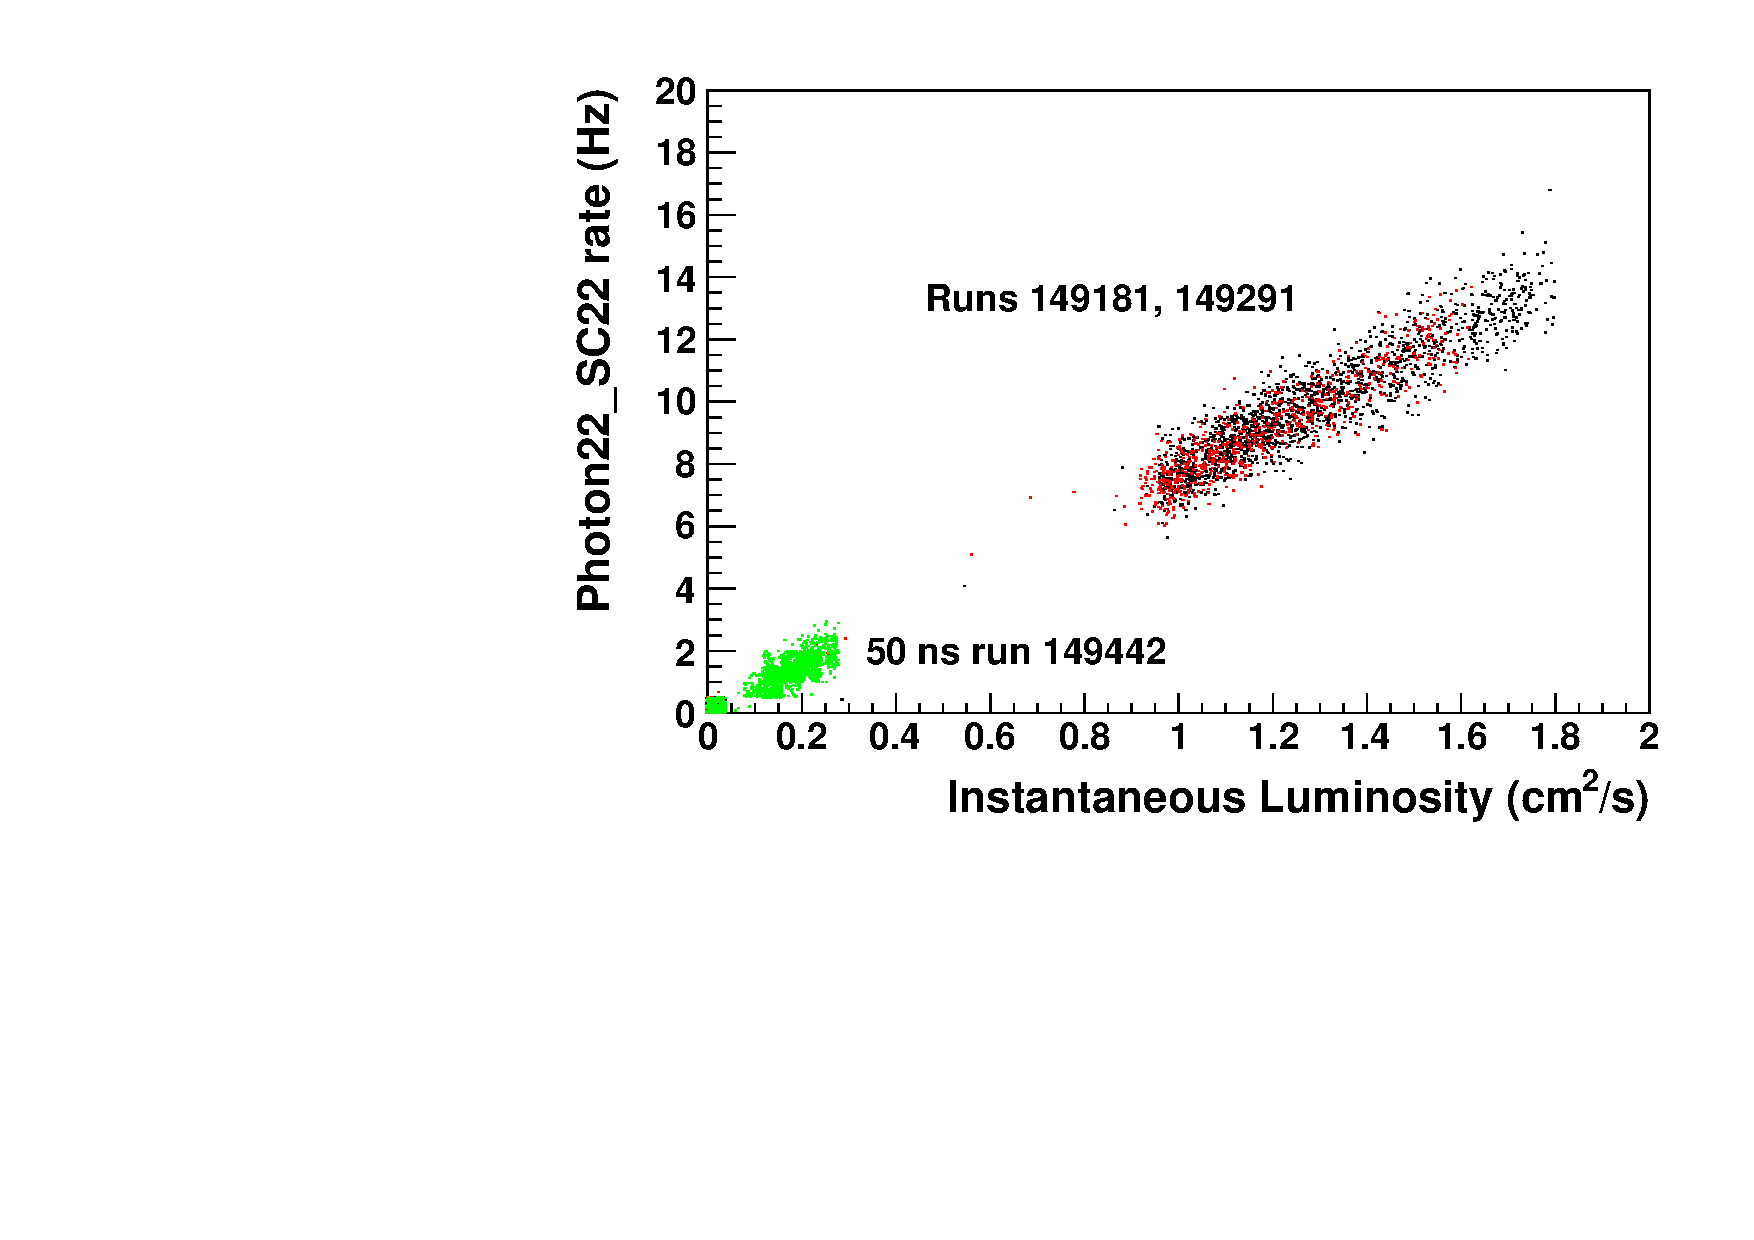
\includegraphics[width=0.85\textwidth]{figures/photon22rates.pdf}
\caption{Scatter plot of HLT\_Photon22\_SC22HE\_L1R trigger rates versus instantaneous luminosity for runs 
149181 (black), 149291 (red) and 149442 (green).  In run149442 the LHC ran with a 50 ns bunch spacing.}
\label{fig:photon22rate}
\end{figure}

Shortly after startup in the upcoming 2011 run, instantaneous luminosity is expected to reach 
$5\times10^{32} cm^2/s$, and in short order top $10^{33} cm^2/s$
later in the spring.  Rates from the triggers relied on last year will be too high to be used unprescaled in 2011. 

Because of the wide variation available in final states produced within GGMSB it is prudent to try to 
cast "as wide a net" as possible to avail detection, while living within rate constraints resulting from 
high luminosity and pile-up.  GGMSB as described above predicts events which in addition to one or more photons 
in the final state, have missing energy due to the exiting gravitino(s) as well
as considerable jet activity.  As the jets in the event can be plentiful but soft $H_T$, the scalar sum
of jet transverse momenta should be a good quantity to trigger by.  With the expected large number of simultaneous
interactions in each event, missing $H_T$, the vector sum of jet transverse momenta above a threshold, is 
expected to be useful for detecting missing energy while being less sensitive to pile-up.  We therefore
concentrate on defining triggers based on photon transverse energy, the $H_T$ of an event, and its $MH_T$.



\section{Trigger rate predictions from data}

One important constraint on trigger definitions is the estimated rate they pass events.  In this
section this is attempted by looking prospective triggers selected from 2010 data, which was 
typically produced with looser triggers than would be needed for 2011.  

\subsection{Trigger descriptions and working points}

In this note we are targetting three quantities by which to trigger -- photon transverse momentum, 
$H_T$:

\begin{equation}
H_T = \sum_{\mathrm{jets} > \mathrm{thresh}} p_T,
\end{equation}

or the scalar sum of jet transverse momentum and missing $H_T$ or $\cancel{H}_T$:

\begin{equation}
\cancel{H}_T = \left| -\sum_{\mathrm{jets} > \mathrm{thresh}} \vec{p}_T \right|,
\end{equation}

which is the vector sum.  Both $H_T$ and $\cancel{H}_T$ are sums for jets above a threshold in $p_T$.  
The thresholds can have the effect of reducing the
effects of beam halo or pile-up.
Initially the threshold for $H_T$ was an uncorrected jet $p_T$ of 20 GeV, and for $\cancel{H}_T$ was 
uncorrected jet $p_T$ of 30 GeV.   As trigger studies progressed and the HLT moved from uncorrected jets
to corrected jets these thresholds evolved to a corrected jet $p_T$ of 40 GeV for $H_T$ and 30 GeV for 
$\cancel{H}_T$.

Photon triggers are defined within a series of "working points" applying different degrees of 
isolation requirements, shown in tables \ref{tab:workingpoints} and \ref{tab:trackandisoworkingpoints}.
Track isolation and the global isolation working points in table \ref{tab:trackandisoworkingpoints}
were not considered here because track isolation is one of the criteria defining "fake" photons
which are expected to be used for background measurements (ref).

\begin{table}
\begin{center}
\begin{tabular}{|lcc|}\hline
Working Point & "CaloId" & "CaloIso" \\ \hline \hline
Very Loose (VL) &  $H/E < 0.15 (0.10)$  & ecalIso/$E_T < 0.2 (0.2)$  \\
                &  $\sigma_{i\eta i\eta} < 0.024 (0.040) $ & hcalIso/$E_T < 0.2 (0.2) $ \\ \hline
Loose (L)       &  $H/E < 0.15 (0.10)$  & ecalIso/$E_T < 0.2 (0.2) $ \\
                &  $\sigma_{i\eta i\eta} < 0.014 (0.035)$  & hcalIso/$E_T < 0.2 (0.2) $ \\ \hline
Tight (T)       &  $H/E < 0.10 (0.075) $ & ecalIso/$E_T < 0.125 (0.125)$  \\
                &  $\sigma_{i\eta i\eta} < 0.011 (0.031) $ & hcalIso/$E_T < 0.125 (0.075) $ \\ \hline
Very Tight (VT) &  $H/E < 0.05 (0.05)$  & ecalIso/$E_T < 0.125 (0.125) $  \\
                &  $\sigma_{i\eta i\eta} < 0.011 (0.031) $ & hcalIso/$E_T < 0.125 (0.075) $  \\ \hline 
\end{tabular}
\end{center}
\caption{Egamma calo ID and isolation operating points, given for the barrel and endcap in parentheses.}
\label{tab:workingpoints}
\end{table}


\begin{table}
\begin{center}
\begin{tabular}{|lccc|}\hline
Working Point & "TrkId" & "TrkIso"  & "Iso" \\ \hline \hline
                 &                       &   & Ecal $E_T < 6.0 + 0.012E_T$  \\
Very Loose (VL)  & $d\eta < 0.01 (0.01)$ & trkIso/$E_T < 0.2 (0.2)$ & Hcal $E_T < 4.0 + 0.005E_T$\\
                 & $d\phi < 0.15 (0.10)$ &  &trk $p_T < 4.0 + 0.002E_T$\\ \hline
                 &                        &               & Ecal $E_T < 5.5 + 0.012E_T$\\
Loose (L) & $d\eta < 0.01 (0.01)$ & trkIso/$E_T < 0.2 (0.2)$& Hcal $E_T < 3.5 + 0.005E_T$\\
                & $d\phi < 0.15 (0.10)$ & & trk $p_T < 3.5 + 0.002E_T$\\ \hline
                                 &                 &                &  Ecal $E_T < 5.0 + 0.012E_T$\\
Tight (T) & $d\eta < 0.008 (0.008) $& trkIso/$E_T < 0.125 (0.075)$& Hcal $E_T < 3.0 + 0.005E_T$\\
                & $d\phi < 0.07 (0.05)$ & &trk $p_T < 3.0 + 0.002E_T$\\ \hline
                 &                 &              &    \\
Very Tight (VT) & $d\eta < 0.008 (0.008)$ & trkIso/$E_T < 0.125 (0.075)$&  - \\
                & $d\phi < 0.07 (0.05) $& &\\ \hline 
\end{tabular}
\end{center}
\caption{Egamma tracker trigger operating points, given for the barrel and endcap in parentheses.  The "Iso"
column refers to global isolation working points, in the trigger path: "IsoVL", "IsoL", and "IsoT" respectively.}
\label{tab:trackandisoworkingpoints}
\end{table}


\subsection{Rates from 2010 Data} 

Trigger rates for proposed dual object triggers were estimated from data in runs (list) and scaled 
to an instantaneous luminosity of $5\times10^32 cm^{-2}/s$.  



\begin{table}
\begin{table}
\begin{center}
\begin{tabular}{|l|ccccccc|}\hline
    & 20 & 22 & 24 & 26 & 28 & 30 & 32 \\ \hline \hline
20 & 37 & 36 & 32 & 29 & 26 & 23 & 21 \\
22 &    & 29 & 27 & 25 & 22 & 20 & 18 \\
24 &    &    & 21 & 19 & 18 & 16 & 15 \\
26 &    &    &    & 15 & 14 & 13 & \bf{12} \\
28 &    &    &    &    & 11 & 11 & 10 \\
30 &    &    &    &    &    & 8  & 8  \\
32 &    &    &    &    &    &    & \bf{6}  \\
\end{tabular}
\end{center}
\caption{Diphoton trigger rates at 5e32 with some kind of isolation}
\end{table}



\begin{table}
\begin{center}
\begin{tabular}{|l|cccc|}\hline
                                & CaloIdVL & CaloIdL & CaloIDVL\_CaloIsolVL & CaloIDL\_CaloIsoVL \\ \hline
Photon28 + Photon26             &      1.5              &        0.6              &       0.7          &  0.4 \\
Photon32 + Photon26             &      11.5              &       4.9               &      5.3          &  2.7 \\         
Photon32 + Photon32             &      5.8              &        2.6              &       3.1         &  1.6 \\
Photon60 + HT200                &      2.0              &       1.5               &       1.8         &  1.4 \\
Photon70 + HT200                &      11.2              &       8.0               &      10.4        &  7.6   \\
Photon70 + HT300                &      4.6              &        3.1              &       4.1         & 2.9  \\
Photon70 + MHT30                &      9.0              &       6.3               &      8.5          & 6.1  \\
Photon70 + MHT50                &      4.7              &       3.1               &      4.5          & 3.0  \\ \hline
\end{tabular}
\end{center}
\caption{Effect of different photon working points on the various types of trigger's rates}
\end{table}

\begin{table}
\begin{center}
\begin{tabular}{|l|ccccc|}\hline
         & HT200 & HT300 & HT400 & HT500 & HT600 \\ \hline \hline
70\_CaloIDL & 8.5 & 3.1 & 0.8 & 0.3 & 0.1 \\
80\_CaloIDL & 5.5 & 2.4 & 0.7 & 0.3 & 0.1 \\
90\_CaloIDL & 3.2 & 1.8 & 0.6 & 0.2 & 0.1 \\
100\_CaloIDL & 2.3 & 1.4 & 0.6 & 0.2 & 0.1 \\ \hline
70\_CaloIDL\_CaloIsoT & 6.6 & 2.1 & 0.5 & 0.2 & 0.1 \\
80\_CaloIDL\_CaloIsoT & 4.3 & 1.6 & 0.4 & 0.2 & 0.1 \\
90\_CaloIDL\_CaloIsoT & 2.7 & 1.4 & 0.4 & 0.2 & 0.1 \\
100\_CaloIDL\_CaloIsoT & 2.0 & 1.2 & 0.4 & 0.2 & 0.1 \\ \hline
\end{tabular}
\end{center}
\caption{Photon+$H_T$ trigger rates}
\end{table}


\begin{table}
\begin{center}
\begin{tabular}{|l|ccccccc|}\hline
         & MHT30 & MHT40 & MHT50 & MHT60 & MHT70 & MHT80 & MHT90 \\ \hline \hline
70\_CaloIDL & 7.4 & 5.3 & 3.8 & 2.5 & 1.9 & 1.4 & 1.3  \\
80\_CaloIDL & 4.2 & 3.1 & 2.3 & 1.6 & 1.1 & 0.8 & 0.7 \\
90\_CaloIDL & 2.3 & 1.8 & 1.3 & 0.9 & 0.7 & 0.6 & 0.5 \\
100\_CaloIDL & 1.6 & 1.1 & 1.0 & 0.7 & 0.5 & 0.4 & 0.3 \\ \hline
70\_CaloIDL\_CaloIsoT & 6.2 & 4.4 & 3.2 & 2.2 & 1.7 & 1.3 & 1.2 \\
80\_CaloIDL\_CaloIsoT & 3.4 & 2.4 & 1.9 & 1.3 & 1.0 & 0.7 & 0.7 \\
90\_CaloIDL\_CaloIsoT & 2.0 & 1.4 & 1.1 & 0.8 & 0.6 & 0.5 & 0.4 \\
100\_CaloIDL\_CaloIsoT & 1.5 & 1.0 & 0.9 & 0.6 & 0.4 & 0.4 & 0.3 \\ \hline
\end{tabular}
\end{center}
\caption{Photon+$\cancel{H}_T$ trigger rates}
\end{table}


\begin{table}
\begin{center}
\begin{tabular}{|l|ccccccccccccccccc|}\hline 
   & 32 & 34 & 36 & 38 & 40 & 42 & 44 & 46 & 48 & 50 & 52 & 54 & 56 & 58 & 60 & 62 & 64 \\ \hline
26 &  4.7  &    &    &    &    &    &    &    &    &    &    &    &    &    &    &    &   \\   
28 &  3.6  & 3.4   &    &    &    &    &    &    &    &    &    &    &    &    &    &    &   \\   
30 & 3.1   & 2.9   & 2.6   &    &    &    &    &    &    &    &    &    &    &    &    &    &   \\
32 &  2.3  & 2.3   & 2.2   &  1.9  &   &    &    &    &    &    &    &    &    &    &    &    &   \\
34 &    & 1.8   & 1.8   & 1.6   & 1.6   &    &    &    &    &    &    &    &    &    &    &    &   \\
36 &    &    & 1.6   & 1.5   & 1.4   & 1.4   &    &    &    &    &    &    &    &    &    &    &   \\
38 &    &    &    & 1.2   &  1.2  & 1.2   &  1.2  &    &    &    &    &    &    &    &    &    &   \\
40 &    &    &    &    & 1.0   &  1.0  & 1.0   & 1.0   &    &    &    &    &    &    &    &    &   \\
42 &    &    &    &    &    & 0.9   & 0.9   & 0.8   & 0.8   &    &    &    &    &    &    &    &   \\
44 &    &    &    &    &    &    & 0.8   & 0.7   & 0.6   &  0.6  &    &    &    &    &    &    &    \\
46 &    &    &    &    &    &    &    & 0.6   & 0.6   & 0.5   & 0.5   &    &    &    &    &    &   \\
48 &    &    &    &    &    &    &    &    & 0.5   & 0.5   & 0.4   & 0.4   &    &    &    &    &    \\
50 &    &    &    &    &    &    &    &    &    & 0.4   & 0.4   & 0.4   & 0.4   &    &    &    &   \\
52 &    &    &    &    &    &    &    &    &    &    & 0.4   & 0.4   & 0.4   & 0.4   &    &    &   \\
54 &    &    &    &    &    &    &    &    &    &    &    & 0.3   & 0.3   & 0.3   & 0.3   &    &    \\
56 &    &    &    &    &    &    &    &    &    &    &    &    & 0.3   & 0.3   & 0.3   &  0.3  &   \\
58 &    &    &    &    &    &    &    &    &    &    &    &    &    & 0.3   & 0.3   & 0.3   & 0.3  \\
60 &    &    &    &    &    &    &    &    &    &    &    &    &    &    & 0.3   & 0.3   & 0.3  \\
62 &    &    &    &    &    &    &    &    &    &    &    &    &    &    &    & 0.3   &  0.3 \\
64 &    &    &    &    &    &    &    &    &    &    &    &    &    &    &    &    &  0.3  \\ \hline
\end{tabular}
\end{center}
\caption{Photon"X"CaloIdLPhoton"Y"CaloIdL trigger rate estimates in Hz for 5e32.  The horizontal direction is 
the threshold applied to the leading photon, vertical descending direction is the threshold
applied to the trailing photon.  "CaloIdL" refers to the "Loose" cuts shown in table \ref{tab:workingpoints}}
\end{table}





\begin{table}
\begin{center}
\begin{tabular}{|l|ccccc|}\hline
         & HT200 & HT300 & HT400 & HT500 & HT600 \\ \hline \hline
70\_CaloIDL & 8.2 & 2.8 & 0.7 & 0.3 & 0.1  \\
80\_CaloIDL & 5.4 & 2.2 & 0.6 & 0.2 & 0.1 \\
90\_CaloIDL & 3.2 & 1.7 & 0.5 & 0.2 & 0.1 \\
100\_CaloIDL & 2.3 & 1.4 & 0.5 & 0.2 & 0.1 \\ \hline
\end{tabular}
\end{center}
\caption{Photon+$H_T$ trigger rates with a 40 GeV requirement on jets entering the $H_T$ sum.}
\end{table}


\begin{table}
\begin{center}
\begin{tabular}{|l|ccccccc|}\hline
         & MHT30 & MHT40 & MHT50 & MHT60 & MHT70 & MHT80 & MHT90 \\ \hline \hline
70\_CaloIDL  &  7.8 & 6.0 & 4.8 & 3.5 & 2.6 & 2.0 & 1.7 \\
80\_CaloIDL&  4.5 & 3.5 & 2.7 & 2.0 & 1.4 & 1.0& 0.9 \\
90\_CaloIDL & 2.6 & 2.0 & 1.6 & 1.2 & 0.8 & 0.7 & 0.5\\
100\_CaloIDL&  1.8 & 1.4 & 1.1& 0.8 & 0.6 & 0.5 & 0.4  \\ \hline
\end{tabular}
\end{center}
\caption{Photon+$\cancel{H}_T$ trigger rates}
\end{table}

\section{Trigger Proposal}

Tables of triggers here, etc.


 \begin{figure}[!ht]
  \centering
 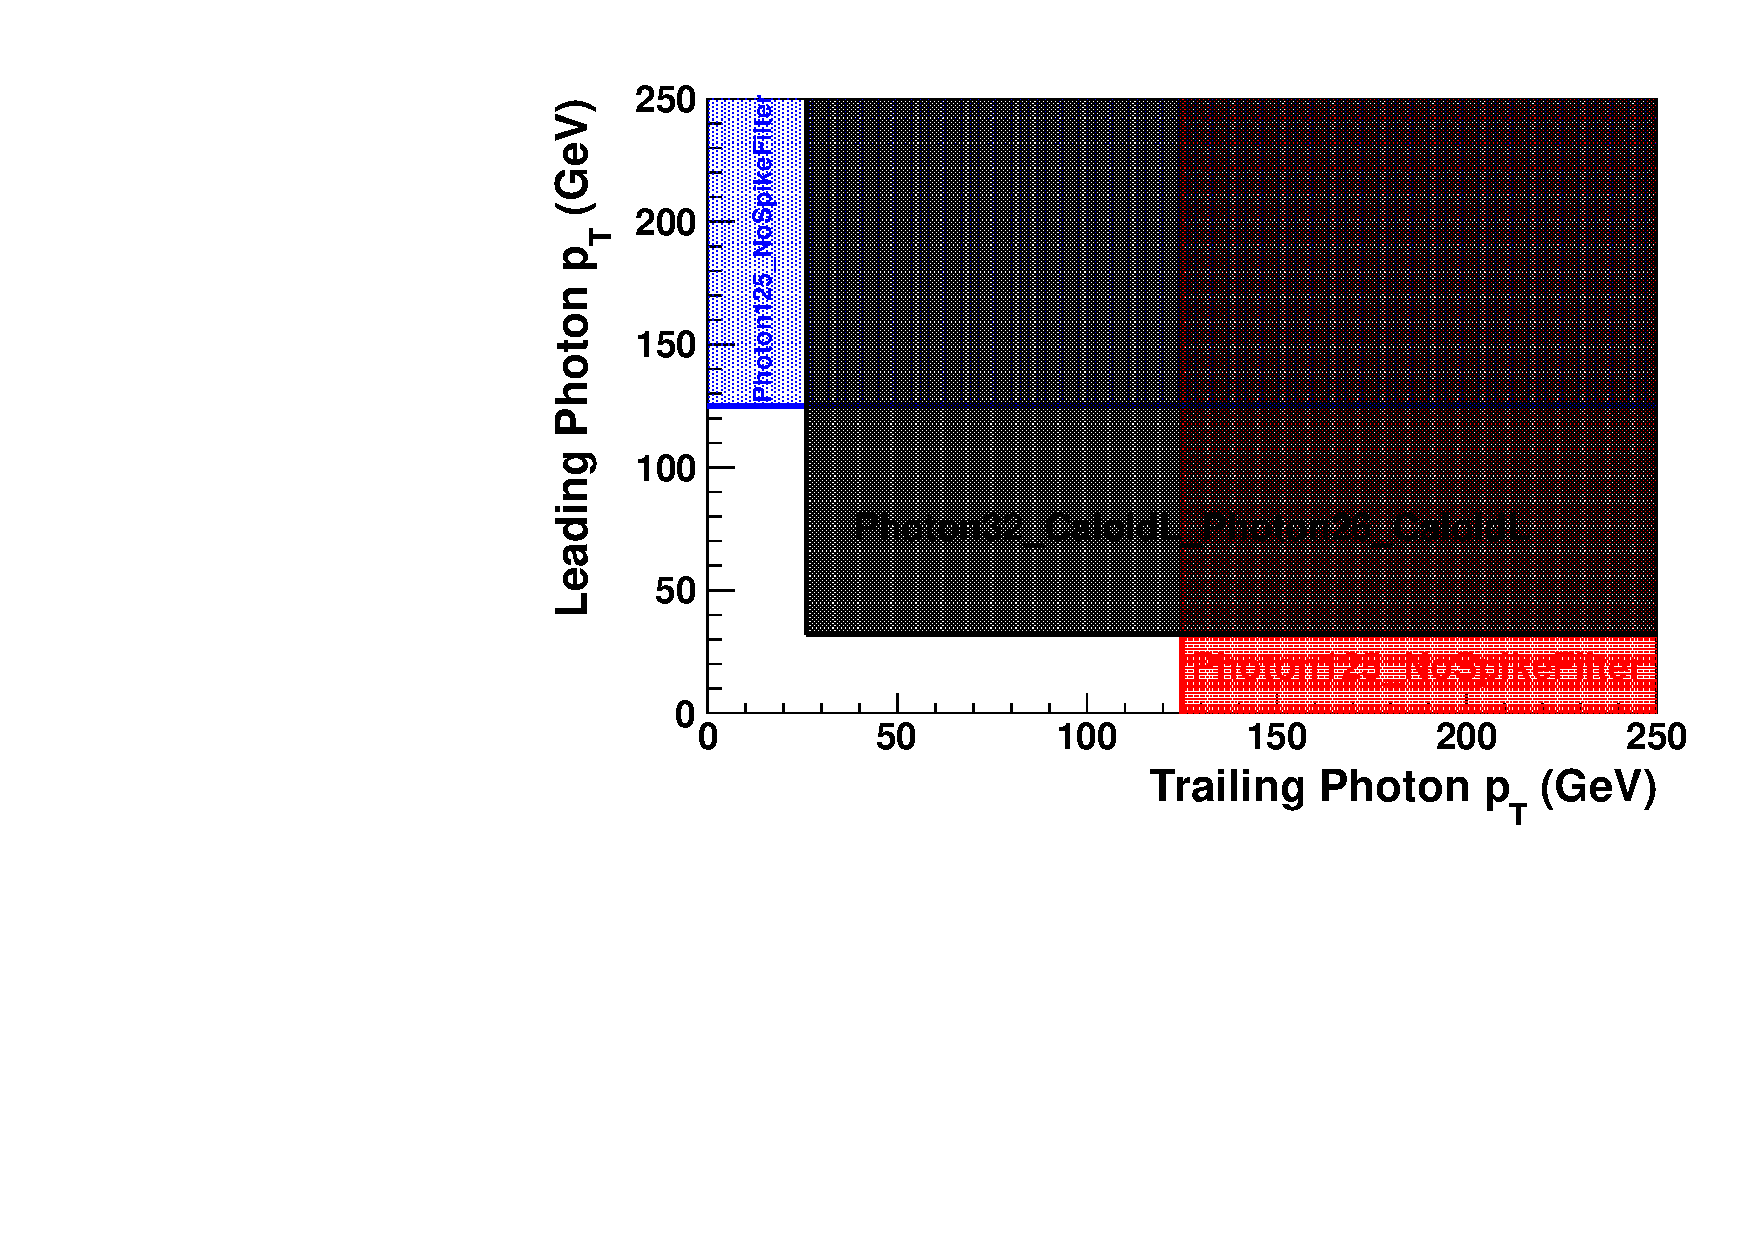
\includegraphics[width=0.90\textwidth]{figures/photonphotonphaseplot.pdf}
\caption{Cartoon of the photon trigger phase space accepted by the single and the proposed diphoton trigger in
the 5E32 trigger menu.}
\label{fig:photonphotonphase}
\end{figure}



 \begin{figure}[!ht]
  \centering
 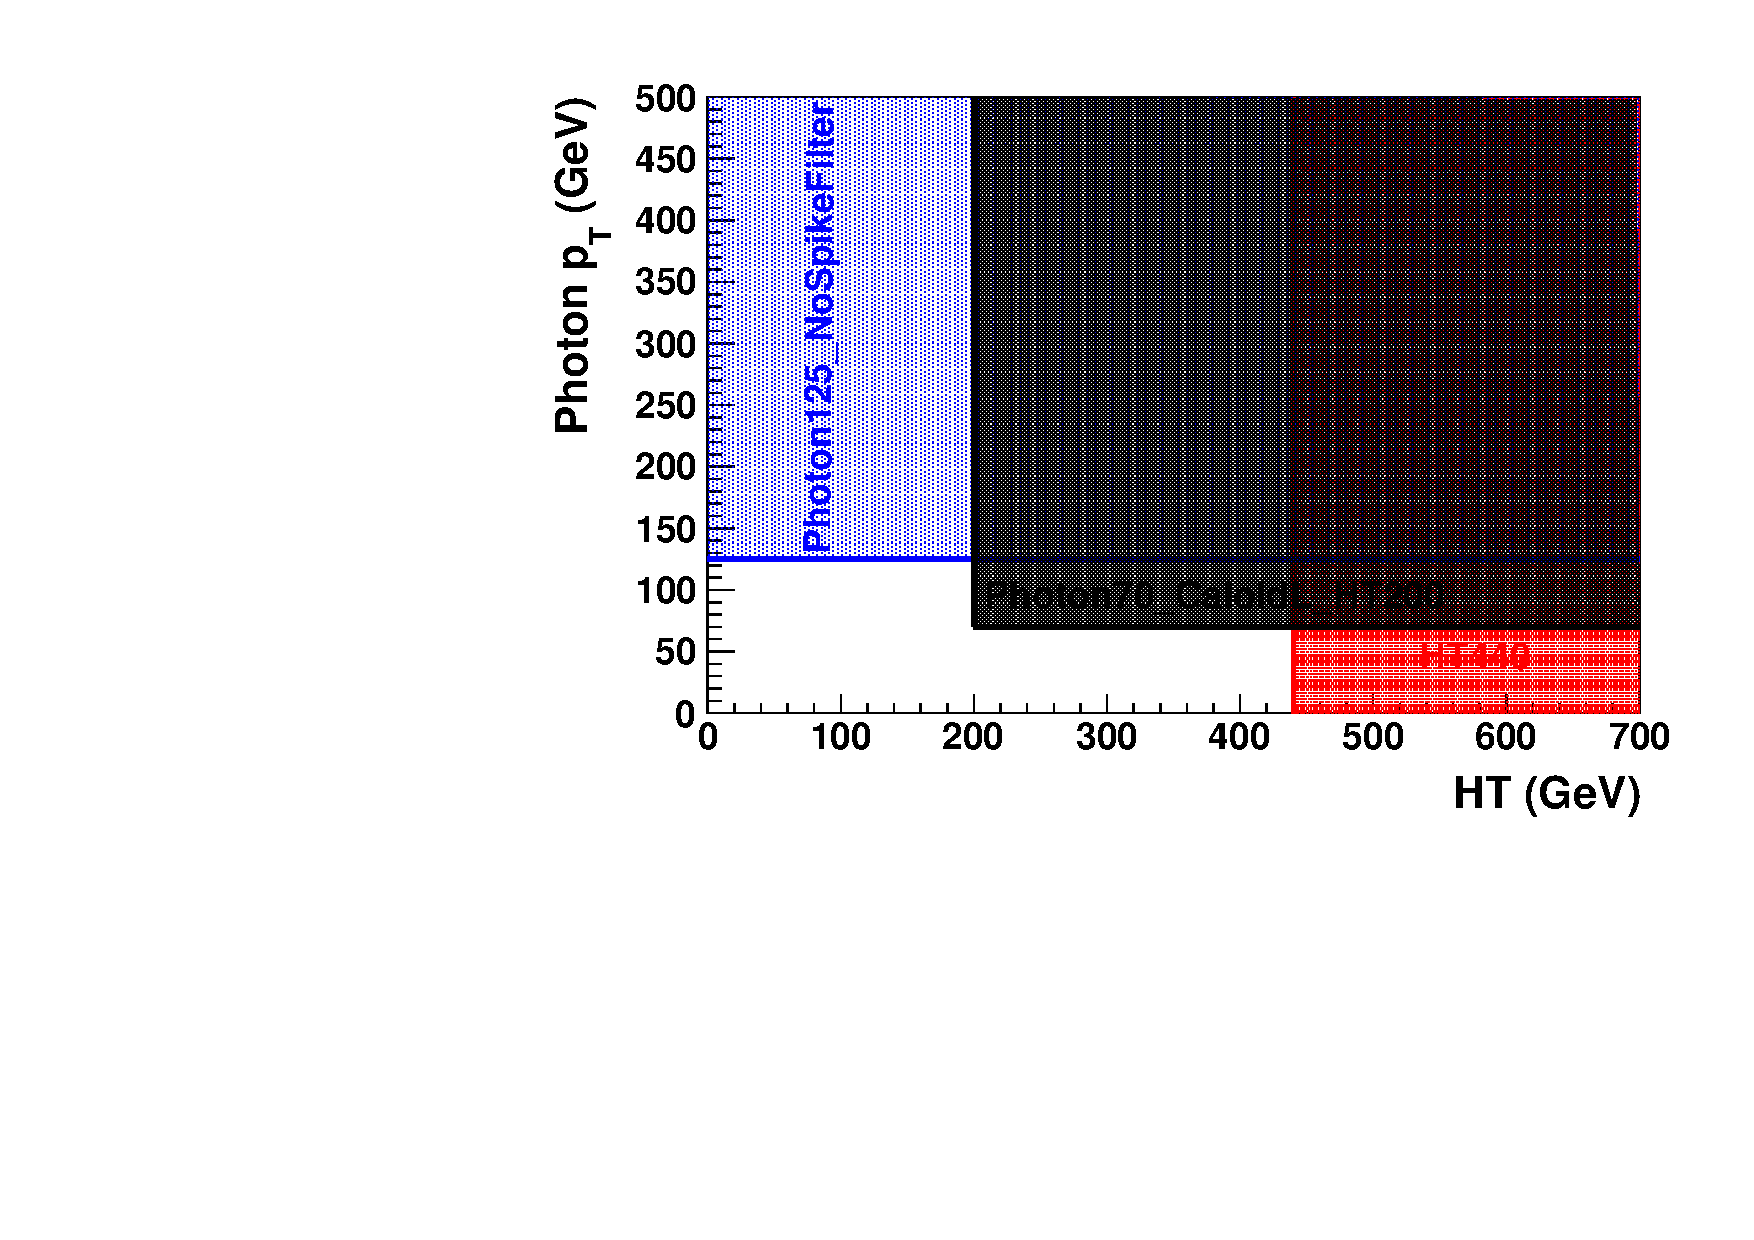
\includegraphics[width=0.90\textwidth]{figures/photon_htphaseplot.pdf}

\caption{Cartoon of the accepted photon+$H_T$  trigger phase space. }
\label{fig:htphase}
\end{figure}

 \begin{figure}[!ht]
  \centering
  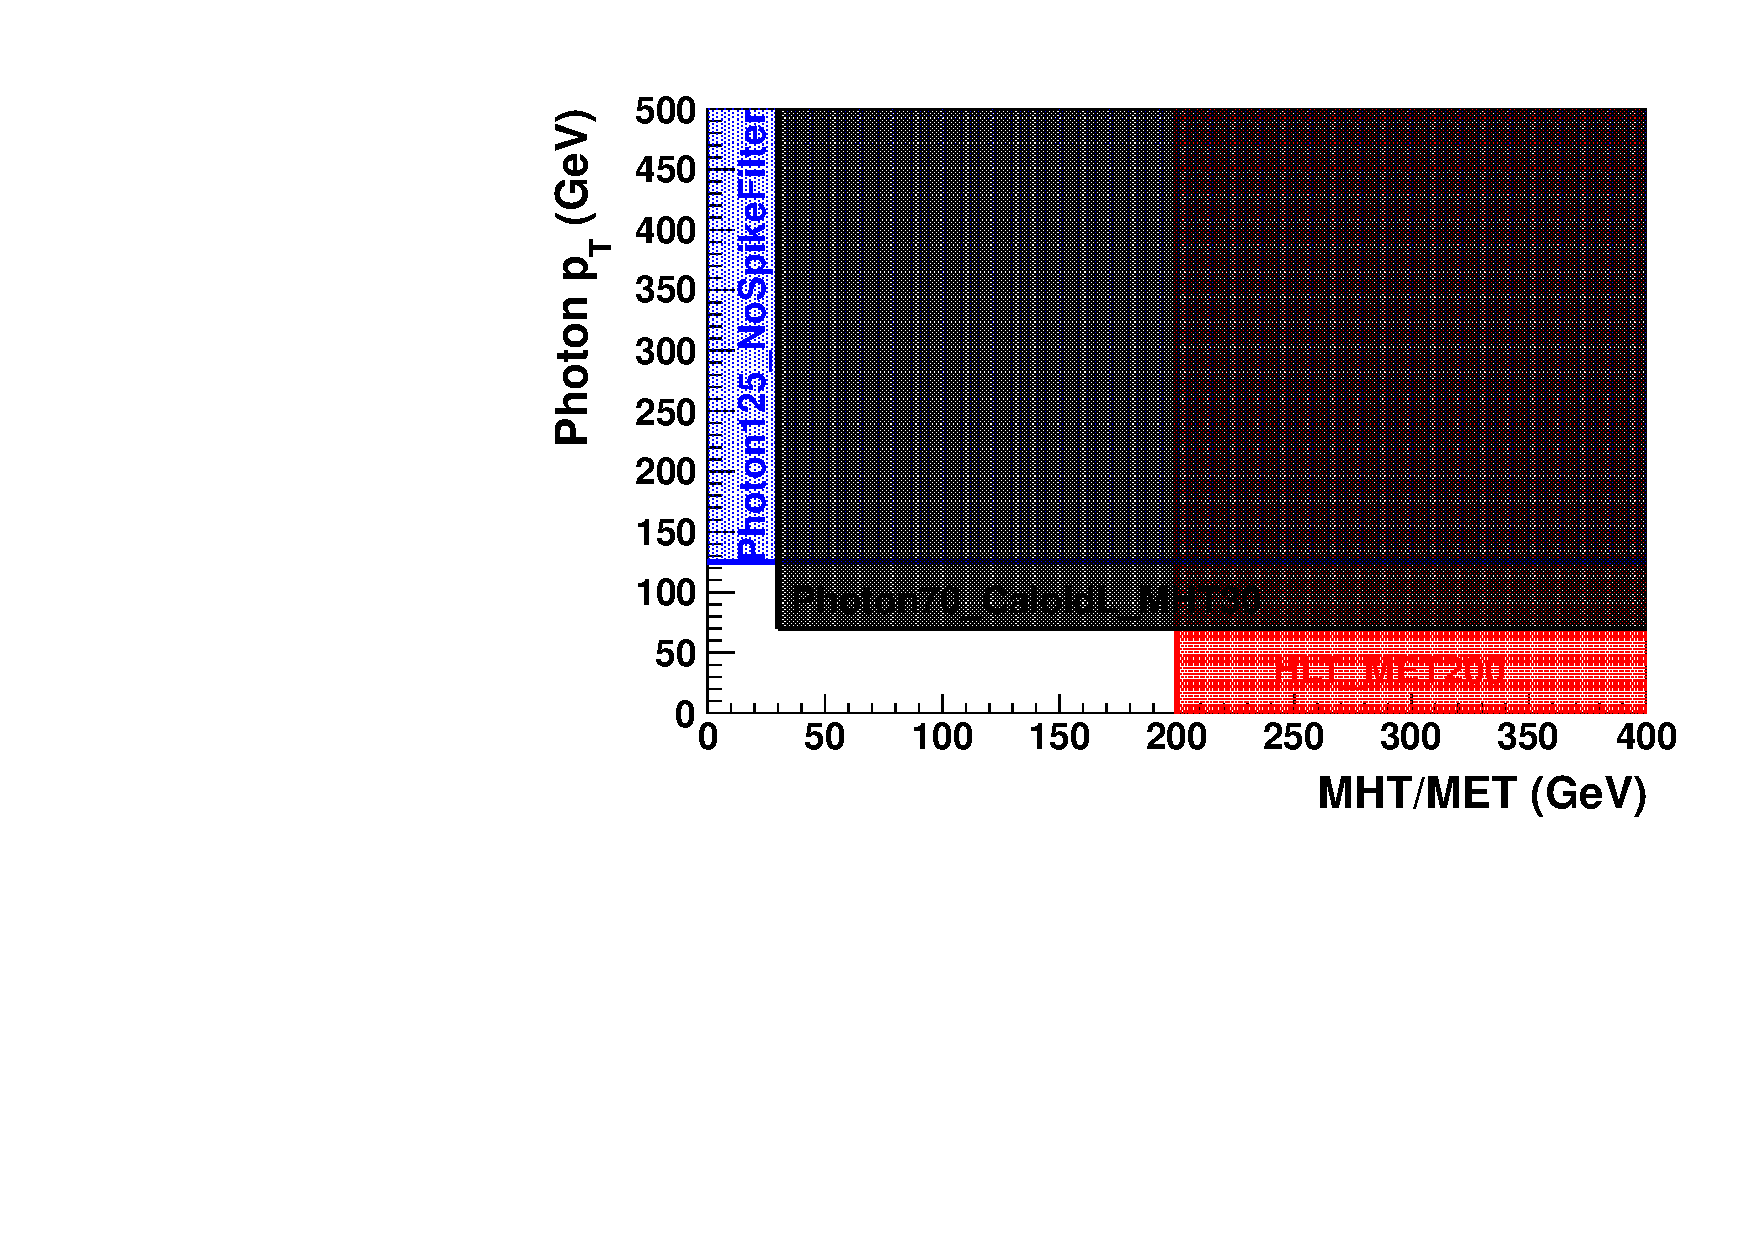
\includegraphics[width=0.90\textwidth]{figures/photon_mhtphaseplot.pdf}
\caption{Cartoon of the accepted photon+MHT trigger phase space. }
\label{fig:mhtphase}
\end{figure}

% Authors: DMason
\section{Signal Acceptance}
\label{sec:signalMC}

Here we look at signal acceptance for 5e32 (and later) triggers.

\subsection{GMSB global acceptance}

SUSY GMSB MC with a coarse grid in $m_{squark}$ = (600,800,1000,1500) GeV, $m_{gluino}$ = (700,900,1200,1600) GeV,
and $m_{wino}$ = (100,300,500) GeV.  The SLHA (ref) SUSY spectra files were generated with SUSPect (ref).
About 2500 events were generated at each grid point and run through the full detector simulation ("fullsim") 
using CMSSW\_3\_11\_1.  For this first study no photon enriching filtering was applied.

Figure \ref{fig:genphotons} shows what percentage of each of these 
generated bins included a generated "prompt" photon from the decay of a $\chi_0$.  One sees fluctuation
between the bins in $m_{squark}$ and $m_{gluino}$ due to statistics in the samples, and a general
trend towards a decreasing percentage of the sample containing prompt photons as the Wino mass increases.
With a Wino mass of 100 GeV the majority of the events include a photon resulting from $\chi_0$ decay.

 \begin{figure}[!ht]
  \centering
 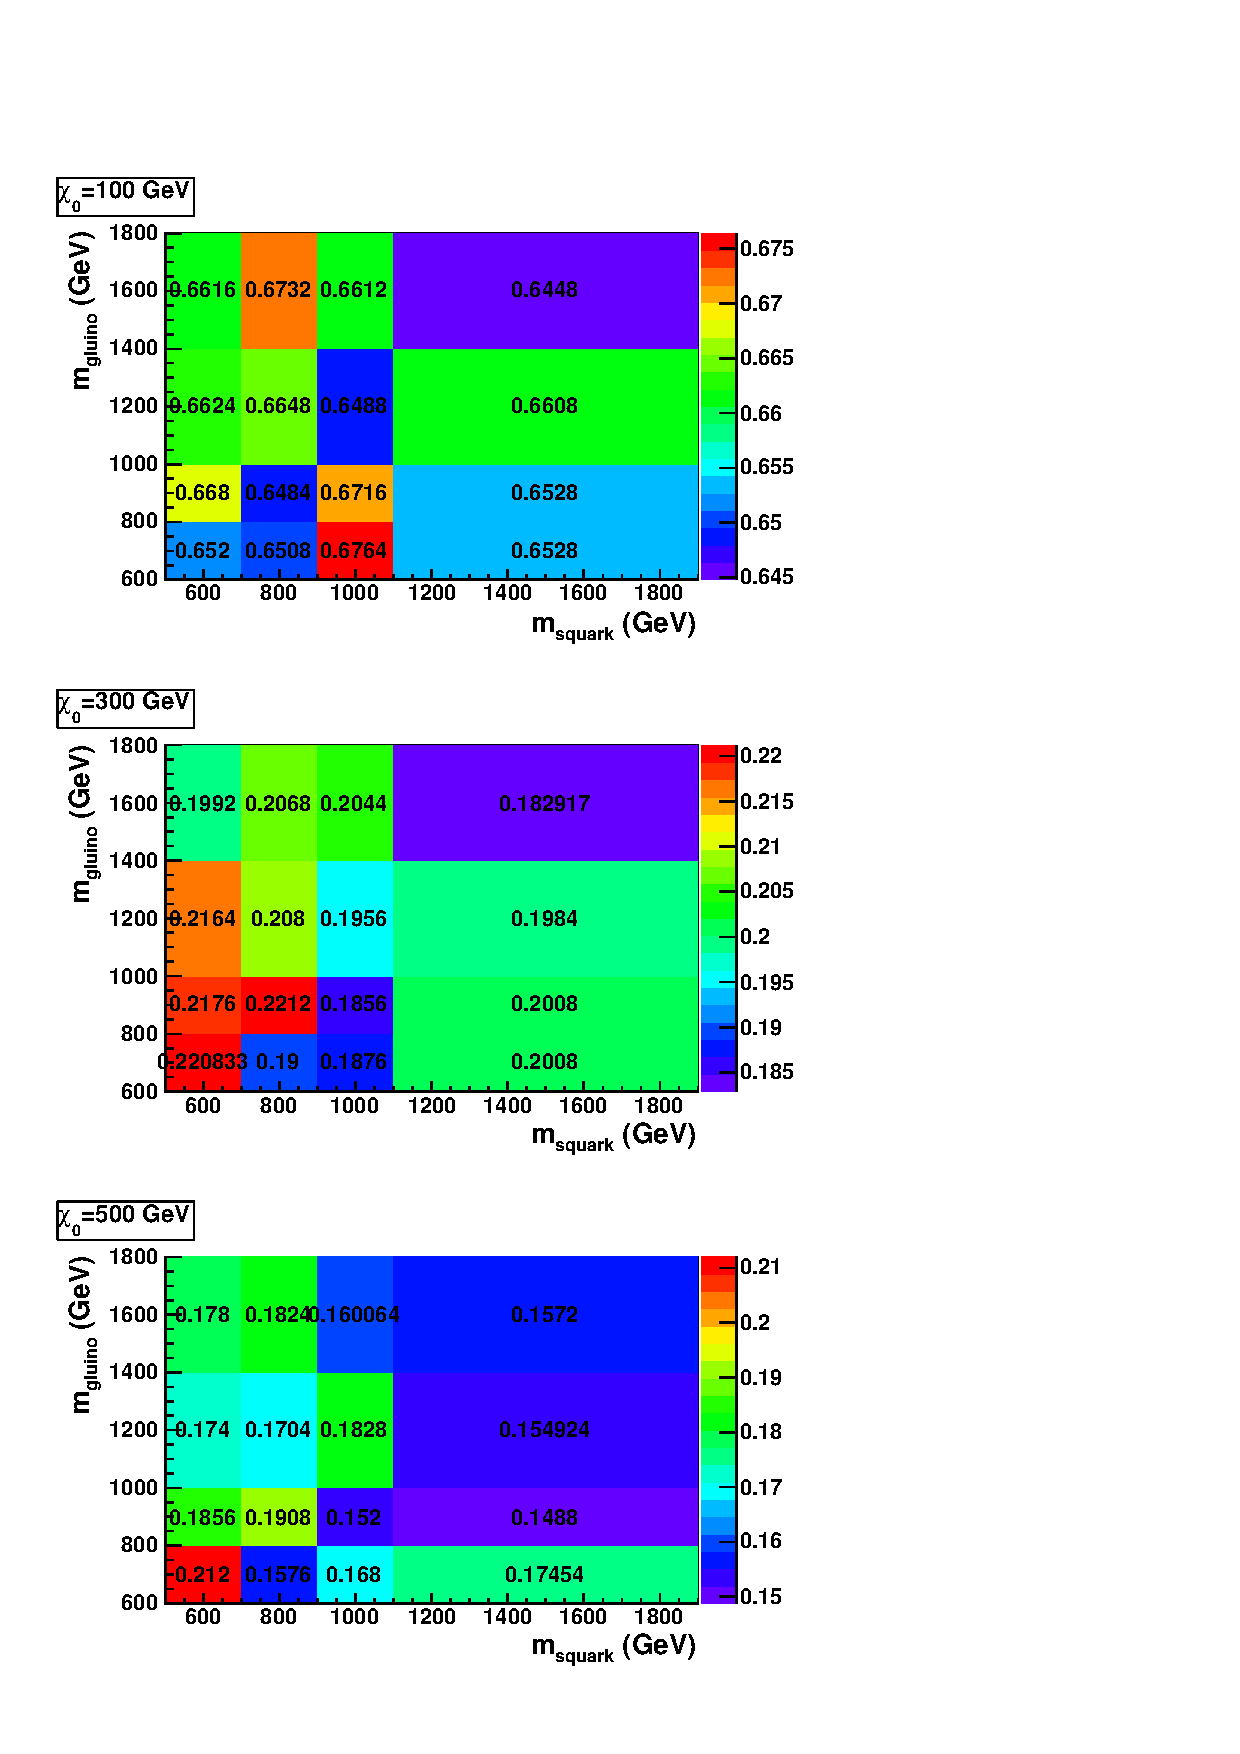
\includegraphics[width=0.5\textwidth]{figures/genphotonsnopu.pdf}
\caption{Percent of MC in each of the 48 bins which have a photon originating from a $\chi_0$.  The three
plots correspond to each of the three Wino mass bins.}
\label{fig:genphotons}
\end{figure}



\subsubsection{SUSY proposed triggers}

 \begin{figure}[!ht]
  \centering
 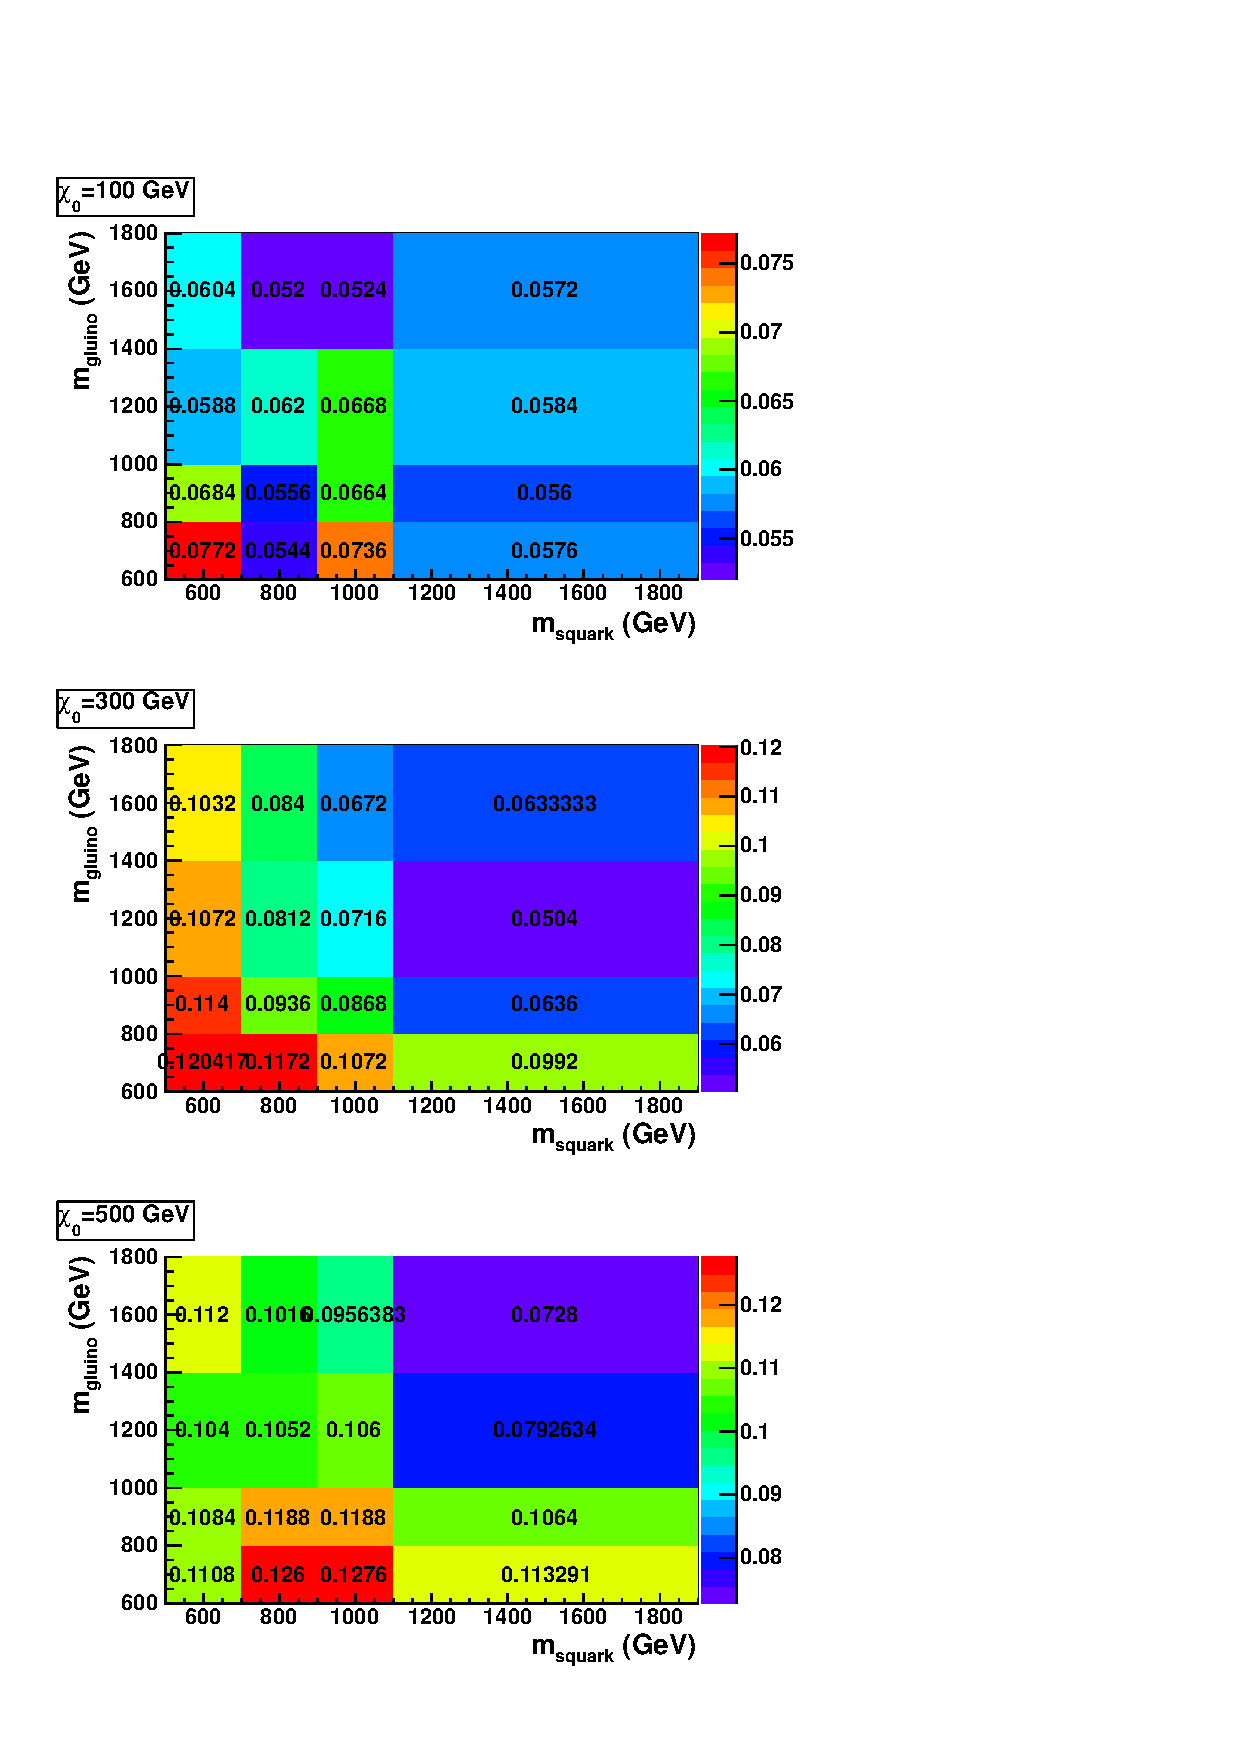
\includegraphics[width=0.45\textwidth]{figures/trigPhoton3226.pdf}
 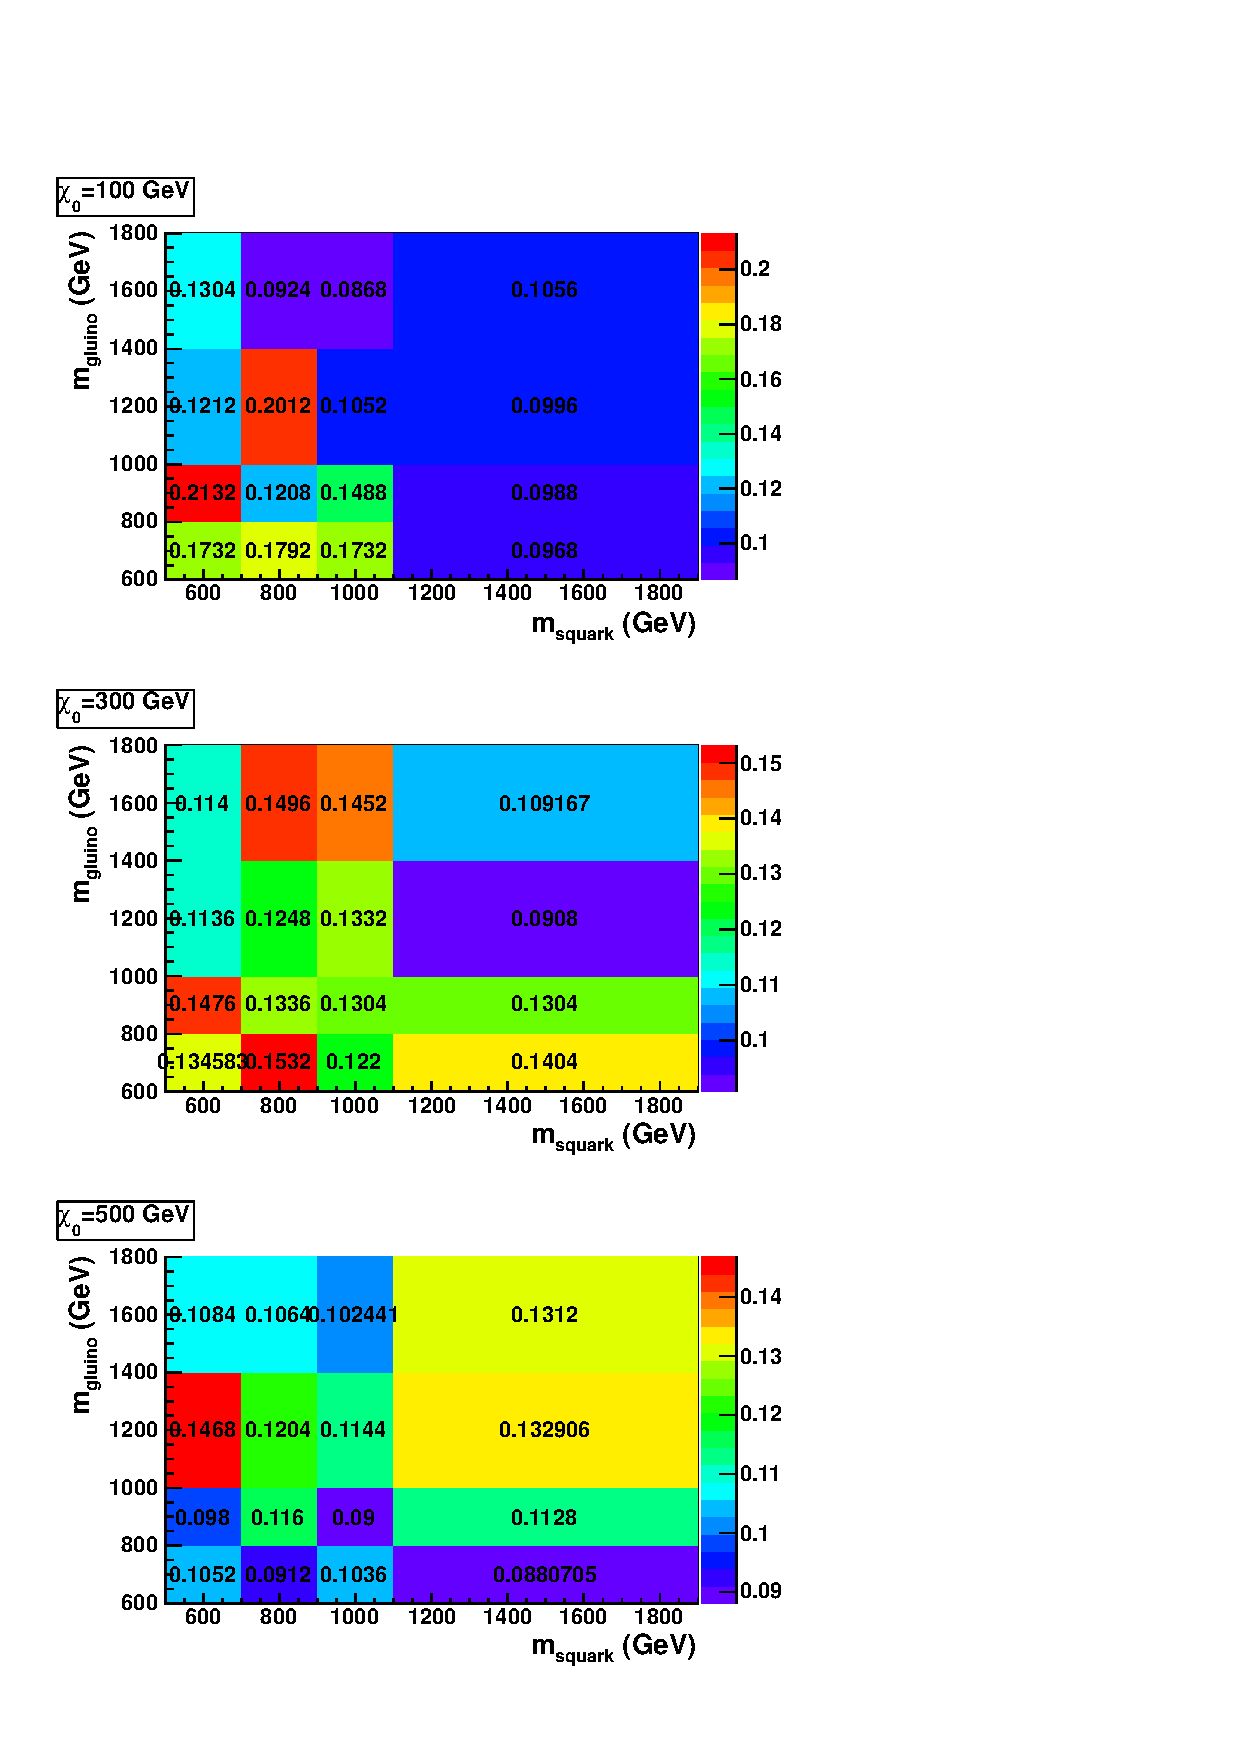
\includegraphics[width=0.45\textwidth]{figures/Photon3226.pdf}

\caption{Percent of MC in each of the 48 bins which pass the HLT\_Photon32\_Photon26\_CaloIdL\_v1 trigger 
(left) and an offline selection of a 32 GeV and 26 GeV photon with calorimeter isolation imposed}
\label{fig:diphotrigs}
\end{figure}

 \begin{figure}[!ht]
  \centering
 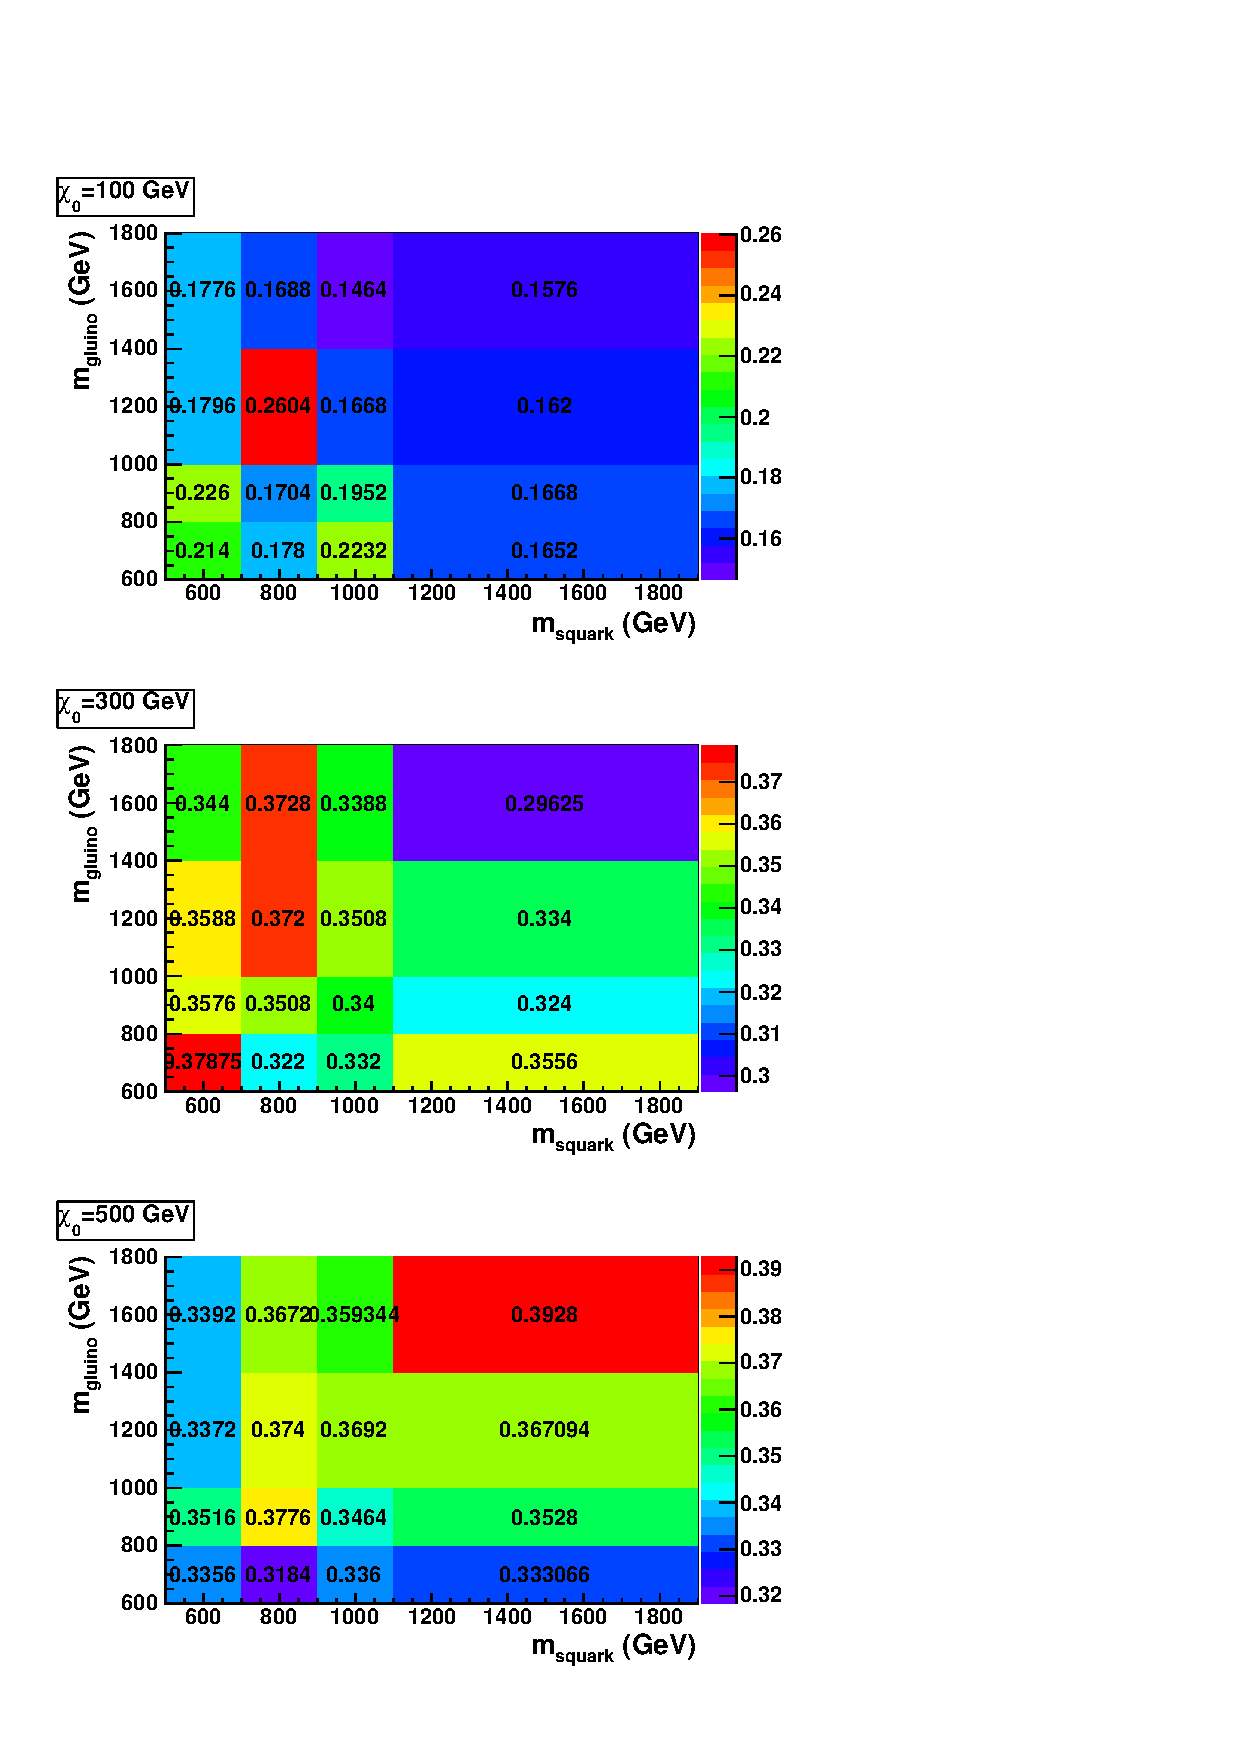
\includegraphics[width=0.45\textwidth]{figures/Photon70MHT30noPU.pdf}
 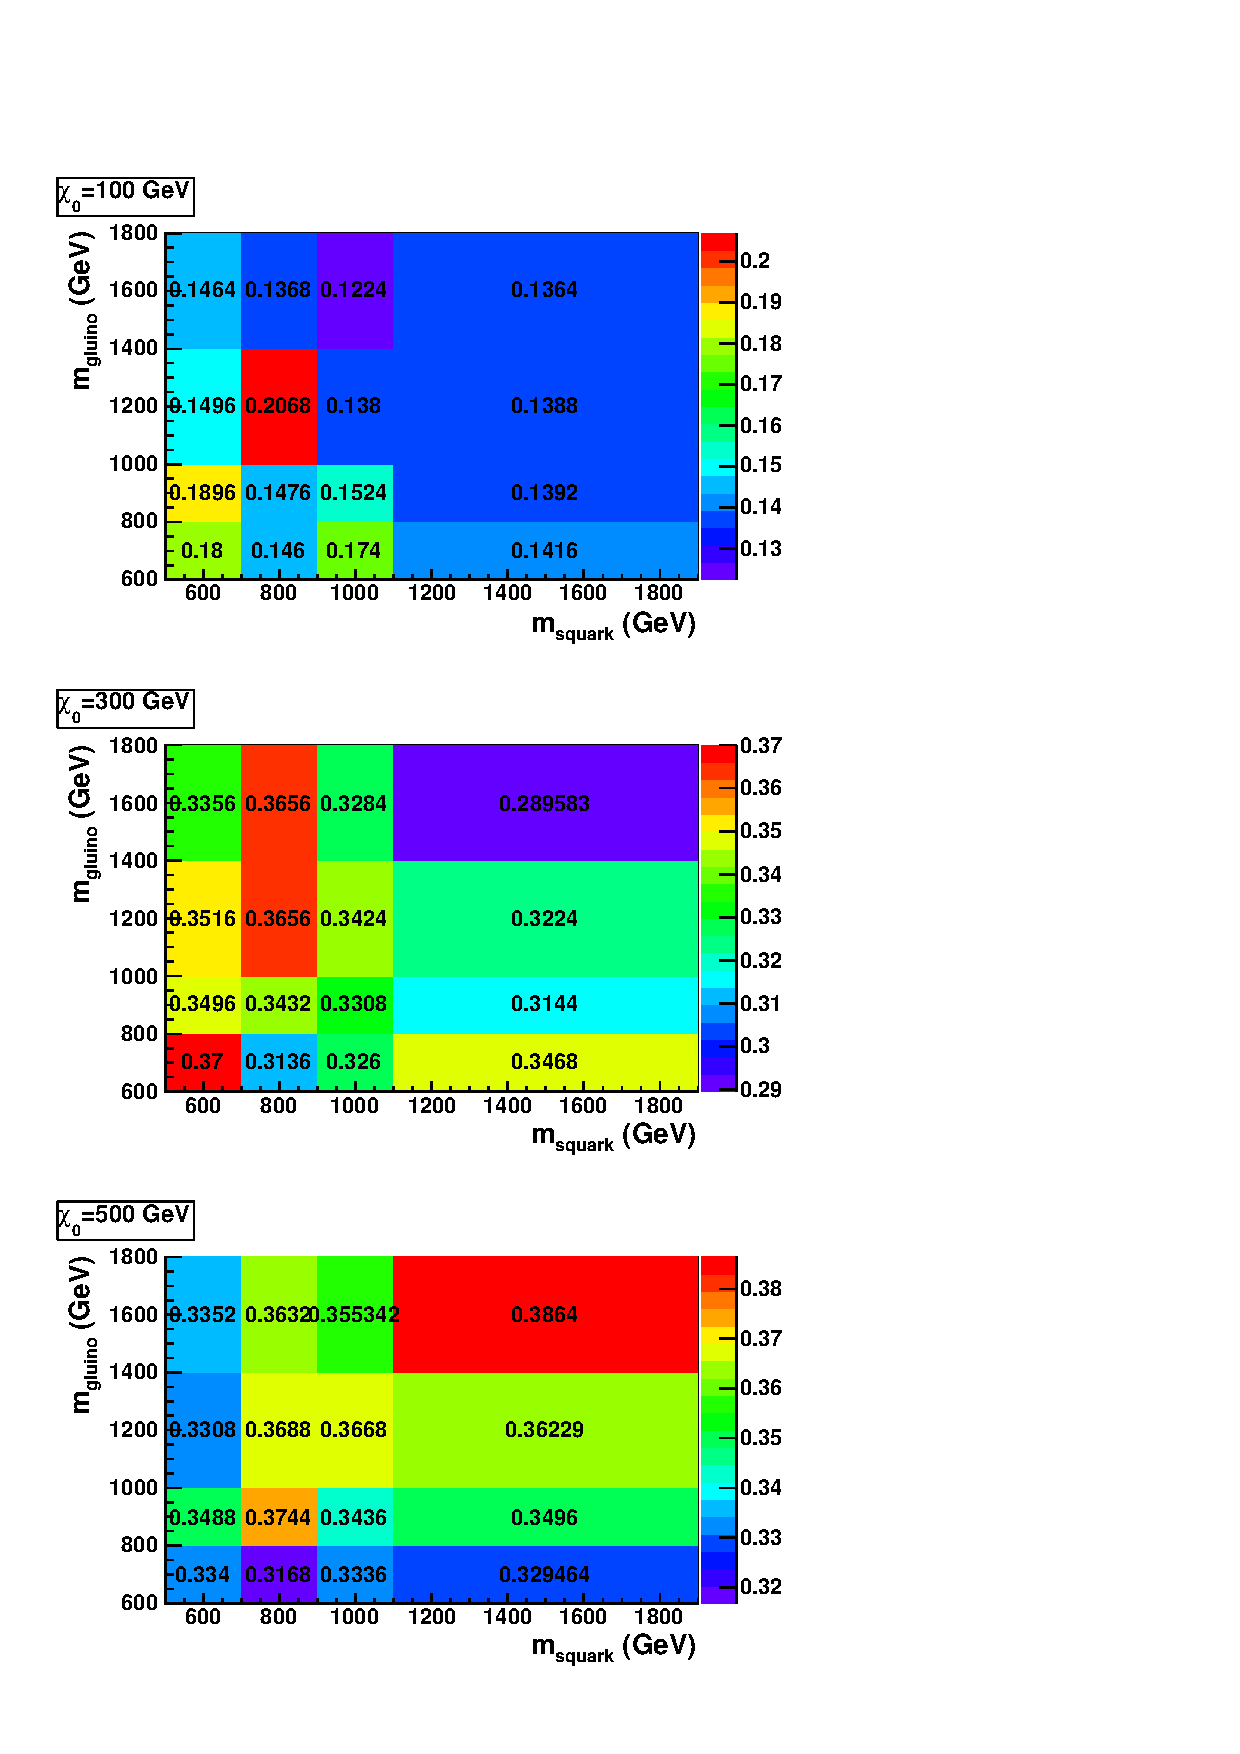
\includegraphics[width=0.45\textwidth]{figures/Photon70MHT50noPU.pdf}

\caption{Percent of MC in each of the 48 bins which pass offline requirements of a 70 GeV photon
and MHT of 30 GeV (left) and 50 GeV (right)}
\label{fig:phomhttrigs}
\end{figure}

 \begin{figure}[!ht]
  \centering
 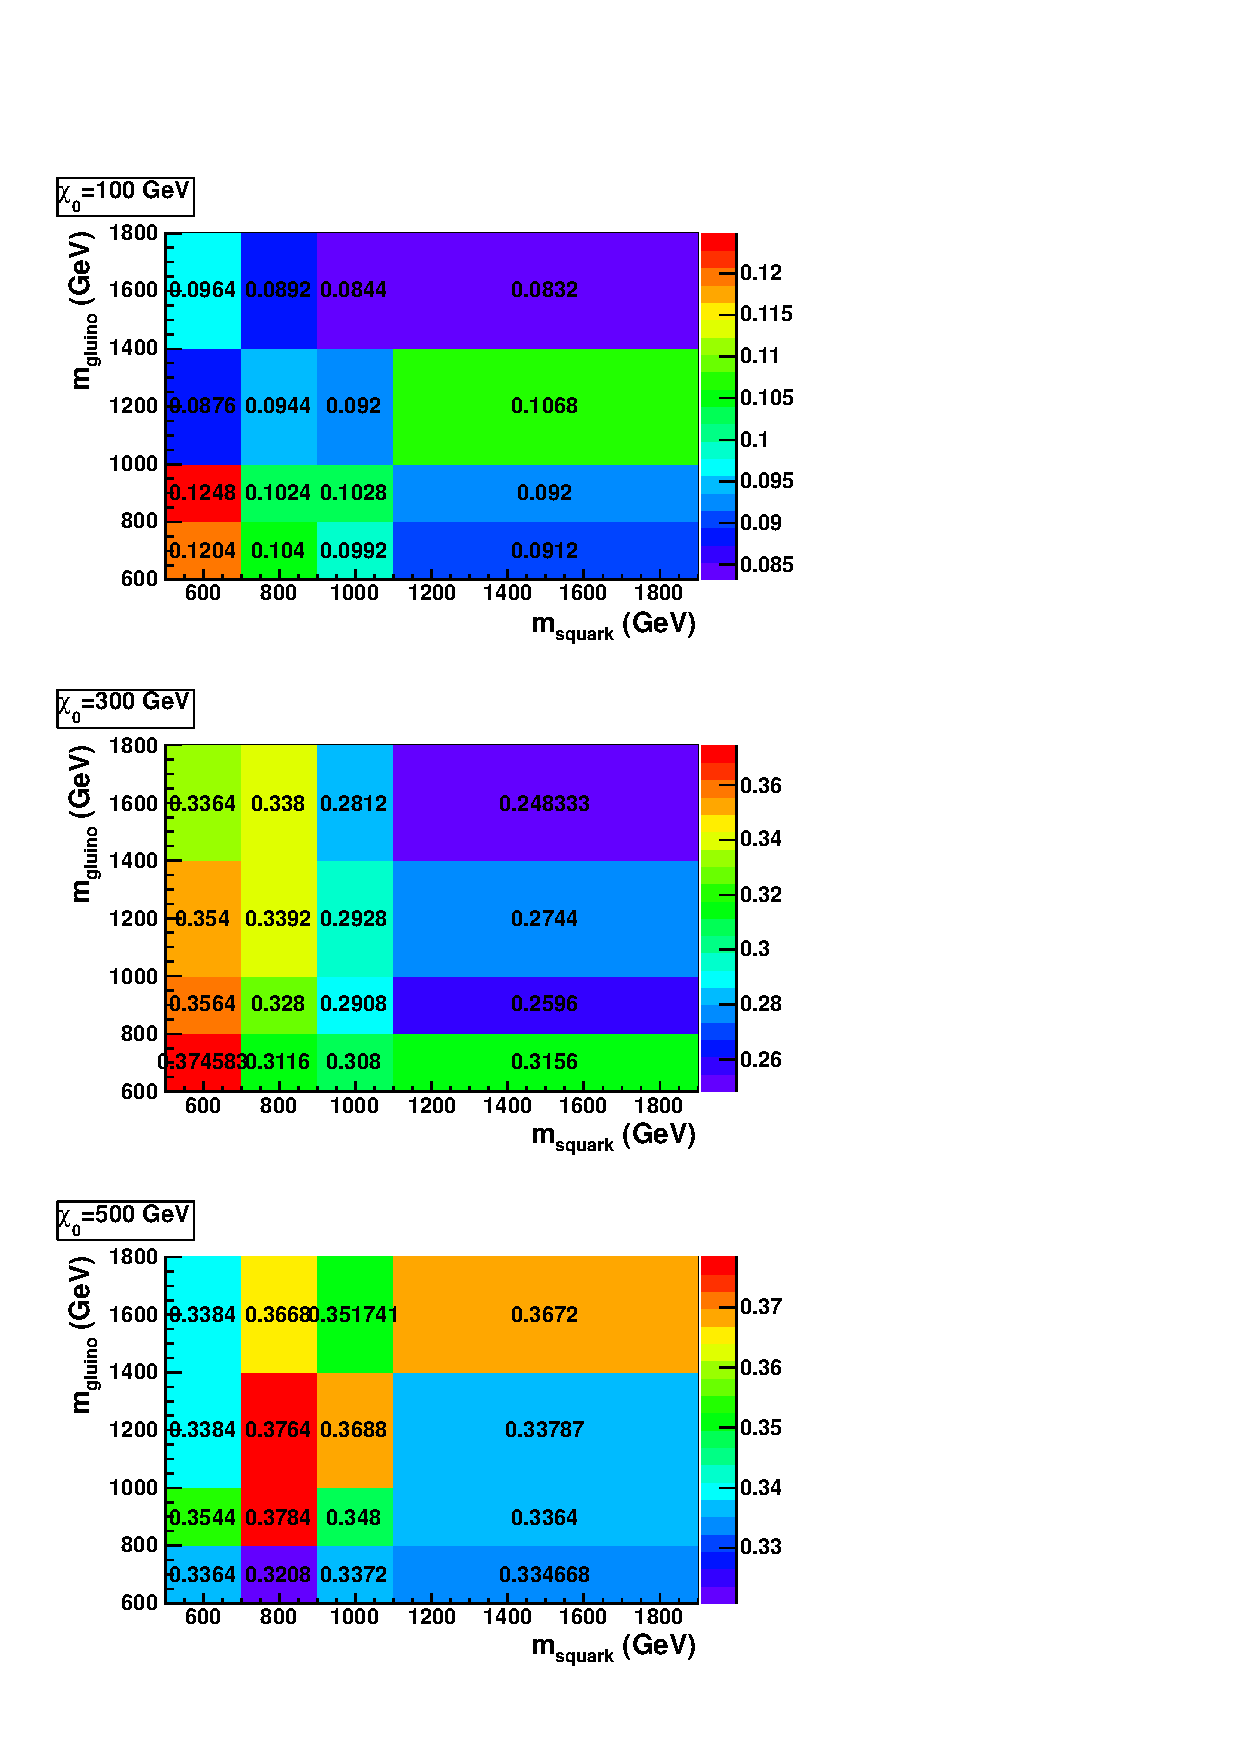
\includegraphics[width=0.45\textwidth]{figures/Photon70HT200noPU.pdf}
 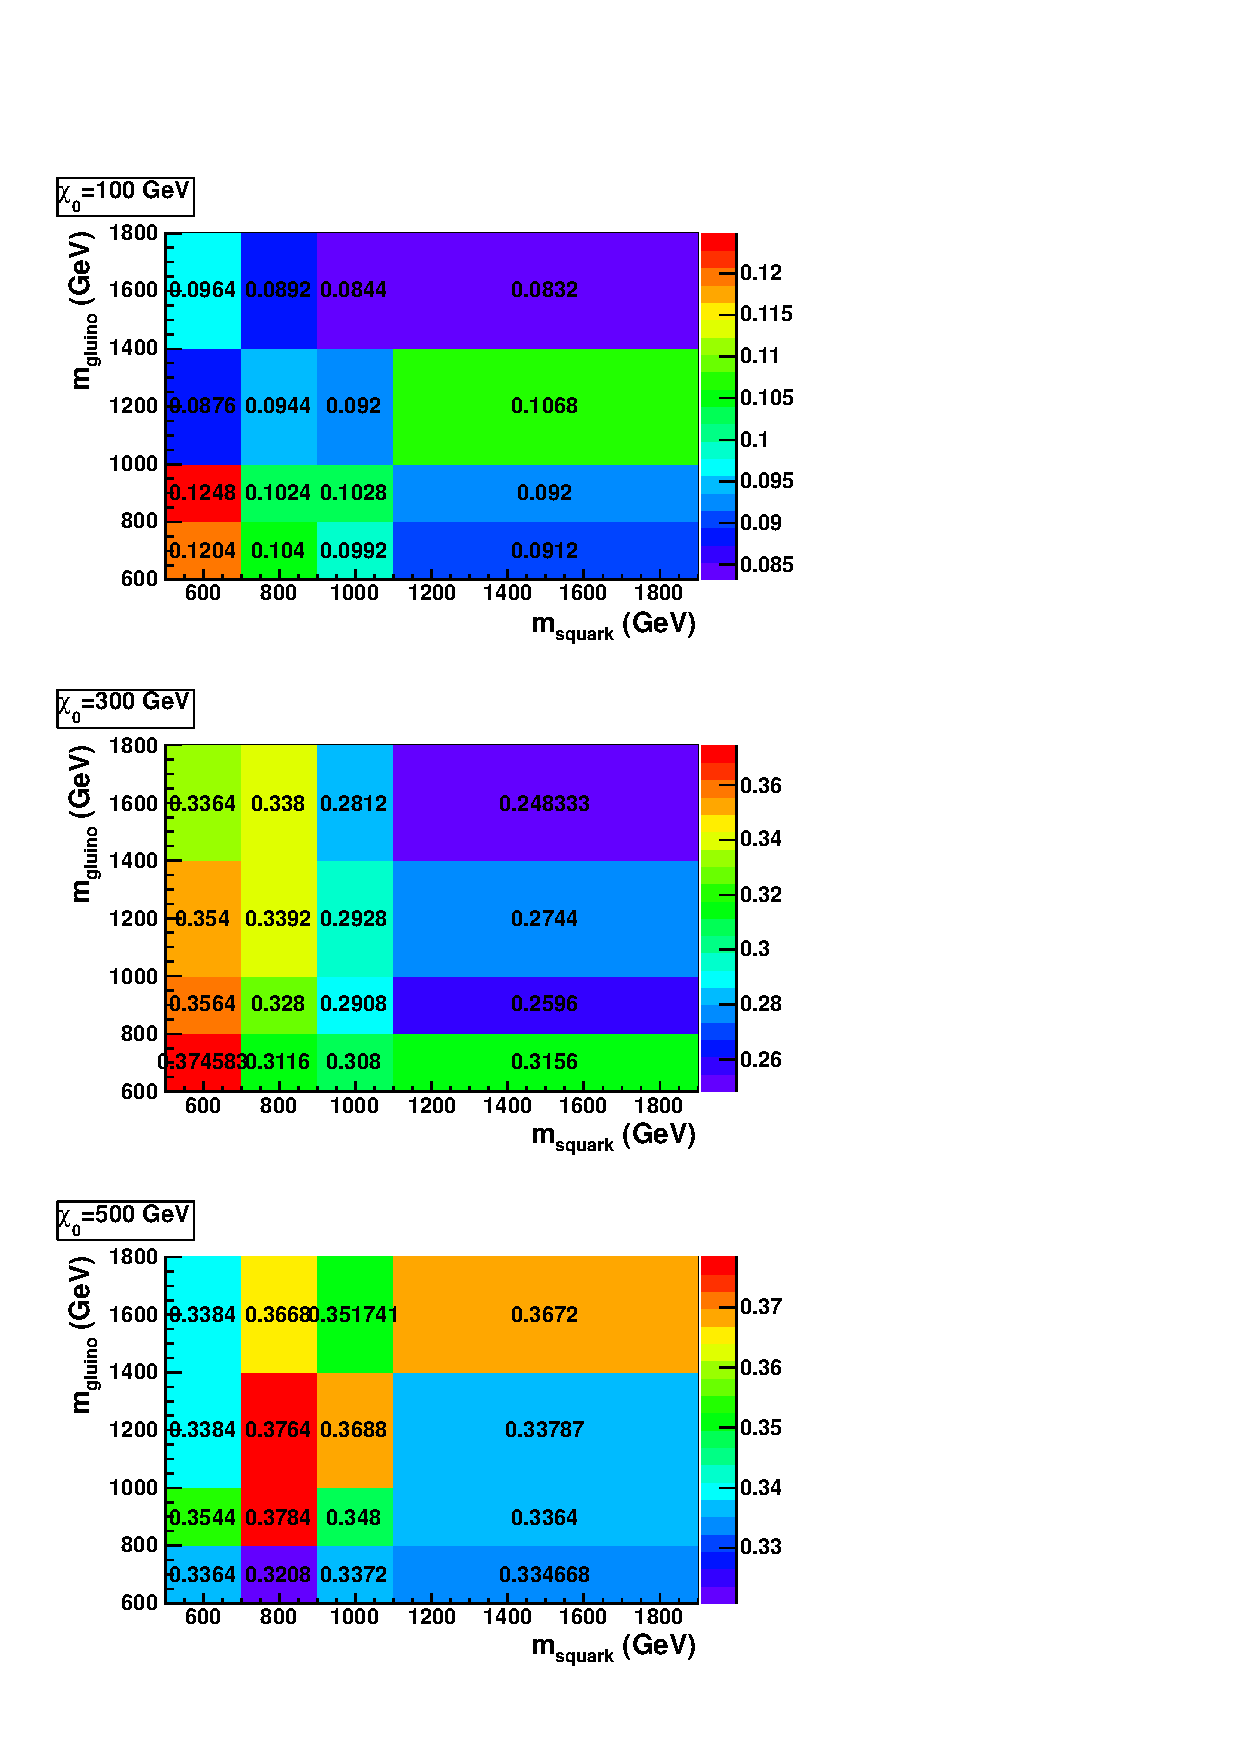
\includegraphics[width=0.45\textwidth]{figures/Photon70HT300noPU.pdf}

\caption{Percent of MC in each of the 48 bins which pass offline requirements of a 70 GeV photon
and HT of 200 GeV (left) and 300 GeV (right)}
\label{fig:phohttrigs}
\end{figure}


\subsubsection{Other useful triggers}




\section{Pile-up Effects}




%\input{Conclusions}
%\clearpage
%\input{Appendix}
%\clearpage

%
% BibTeX Bibliography
%
% Attention! The following style is already set in the cms-tdr class!
%\bibliographystyle{auto_generated}
% and the following is generated from bib files in the current
% directory PLUS TDR bib files 
%\bibliography{my-references,qcd,ptdr2,auto_generated}
\bibliography{auto_generated,my-references,qcd}

% For use with the tdr script comment \end{document} 
\end{document}
